%% LLT: Turn off some annoying warnings...
\RequirePackage{silence}
\WarningFilter{titlesec}{Non standard sectioning command}
\WarningFilter{scrreprt}{Usage of package}
\WarningFilter{scrreprt}{Activating an ugly workaround}

% **************************************************
% Document Class Definition
% **************************************************
\documentclass[%
	paper=A4,					% paper size --> A4 is default in Germany
	twoside=true,				% onesite or twoside printing
	openright,					% doublepage cleaning ends up right side
	parskip=full,				% spacing value / method for paragraphs
	chapterprefix=true,			% prefix for chapter marks
	11pt,						% font size
	headings=normal,			% size of headings
	bibliography=totoc,			% include bib in toc
	listof=totoc,				% include listof entries in toc
	titlepage=on,				% own page for each title page
	captions=tableabove,		% display table captions above the float env
	draft=false,				% value for draft version
]{scrreprt}%

% **************************************************
% Debug LaTeX Information
% **************************************************
%\listfiles

% **************************************************
% Information and Commands for Reuse
% **************************************************
\newcommand{\thesisTitle}{Bright Galaxies as Redshift Tracers for Dark Siren Cosmology}
\newcommand{\thesisName}{Muhammad Khuzaifa Naveed}
\newcommand{\thesisSubject}{Master Thesis}
\newcommand{\thesisDate}{AY 2024-2025}
\newcommand{\thesisDateSubmission}{June, 2025}
\newcommand{\thesisVersion}{First Draft}

%\newcommand{\thesisFirstReviewer}{Jane Doe}
%\newcommand{\thesisFirstReviewerUniversity}{\protect{Ghent University}}
%\newcommand{\thesisFirstReviewerDepartment}{Department of Clean Thesis %Style}
%
%\newcommand{\thesisSecondReviewer}{John Doe}
%\newcommand{\thesisSecondReviewerUniversity}{\protect{Ghent University}}
%\newcommand{\thesisSecondReviewerDepartment}{Department of Clean Thesis Style}

\newcommand{\thesisFirstSupervisor}{Prof. Dr. Archisman Ghosh}
%\newcommand{\thesisSecondSupervisor}{John Smith}

\newcommand{\thesisUniversity}{\protect{Ghent University}}
\newcommand{\thesisUniversityDepartment}{Department of Physics and Astronomy}
%\newcommand{\thesisUniversityInstitute}{Institut for Clean Thesis Dev}
\newcommand{\thesisUniversityGroup}{Ghent Gravity Group}
\newcommand{\thesisUniversityCity}{Ghent}
\newcommand{\thesisUniversityStreetAddress}{Proeftuinstraat 86}
\newcommand{\thesisUniversityPostalCode}{9000}

% **************************************************
% Load and Configure Packages
% **************************************************
\usepackage{pdfpages}
\usepackage{svg}
\usepackage[printonlyused,withpage]{acronym}
\usepackage{hyperref}
\usepackage{tocloft}
\usepackage[toc,acronym]{glossaries}
\usepackage[utf8]{inputenc}		% defines file's character encoding
\usepackage[english]{babel} % babel system, adjust the language of the content
\usepackage[					% clean thesis style
	figuresep=colon,%
	sansserif=false,%
	hangfigurecaption=false,%
	hangsection=true,%
	hangsubsection=true,%
	colorize=full,%
	colortheme=bluemagenta,%
% LLT: Use biber if using UTF8 encoding
 	bibsys=bibtex,%
%	bibsys=biber,%
	bibfile=bib-refs,%
	bibstyle=authoryear,%
]{cleanthesis}

\hypersetup{					% setup the hyperref-package options
	pdftitle={\thesisTitle},	% 	- title (PDF meta)
	pdfsubject={\thesisSubject},% 	- subject (PDF meta)
	pdfauthor={\thesisName},	% 	- author (PDF meta)
	plainpages=false,			% 	-
	colorlinks=true,			% 	- colorize links?
	pdfborder={0 0 0},			% 	-
	breaklinks=true,			% 	- allow line break inside links
	bookmarksnumbered=true,		%
	bookmarksopen=true,			%
        linkcolor= black,
        anchorcolor = ctcoloraccessory,
        citecolor = ctcoloraccessory,
        filecolor = ctcoloraccessory,
        menucolor = red,
        runcolor = ctcoloraccessory,
        urlcolor = ctcoloraccessory
}

\renewcommand{\cftloftitlefont}{\thesischapterfont\huge\bfseries}
\renewcommand{\cftfigfont}{\helv\normalsize}

\renewcommand{\cftlottitlefont}{\thesischapterfont\huge\bfseries}
\renewcommand{\cfttabfont}{\helv\normalsize}

\renewcommand{\cfttoctitlefont}{\thesischapterfont\huge\bfseries}
\renewcommand{\cftchapfont}{\thesisparagraphfont\normalsize\bfseries}
\renewcommand{\cftsecfont}{\helv}
\renewcommand{\cftsubsecfont}{\helv}
% **************************************************
% Document CONTENT
% **************************************************
\begin{document}

% --------------------------
% rename document parts
% --------------------------
%\renewcaptionname{ngerman}{\figurename}{Abb.}
%\renewcaptionname{ngerman}{\tablename}{Tab.}
\renewcaptionname{english}{\figurename}{Fig.}
\renewcaptionname{english}{\tablename}{Tab.}

% --------------------------
% Front matter
% --------------------------
\pagenumbering{roman}			% roman page numbing (invisible for empty page style)
\pagestyle{empty}				% no header or footers
% !TEX root = ../thesis-example.tex
%
% ------------------------------------  --> cover title page
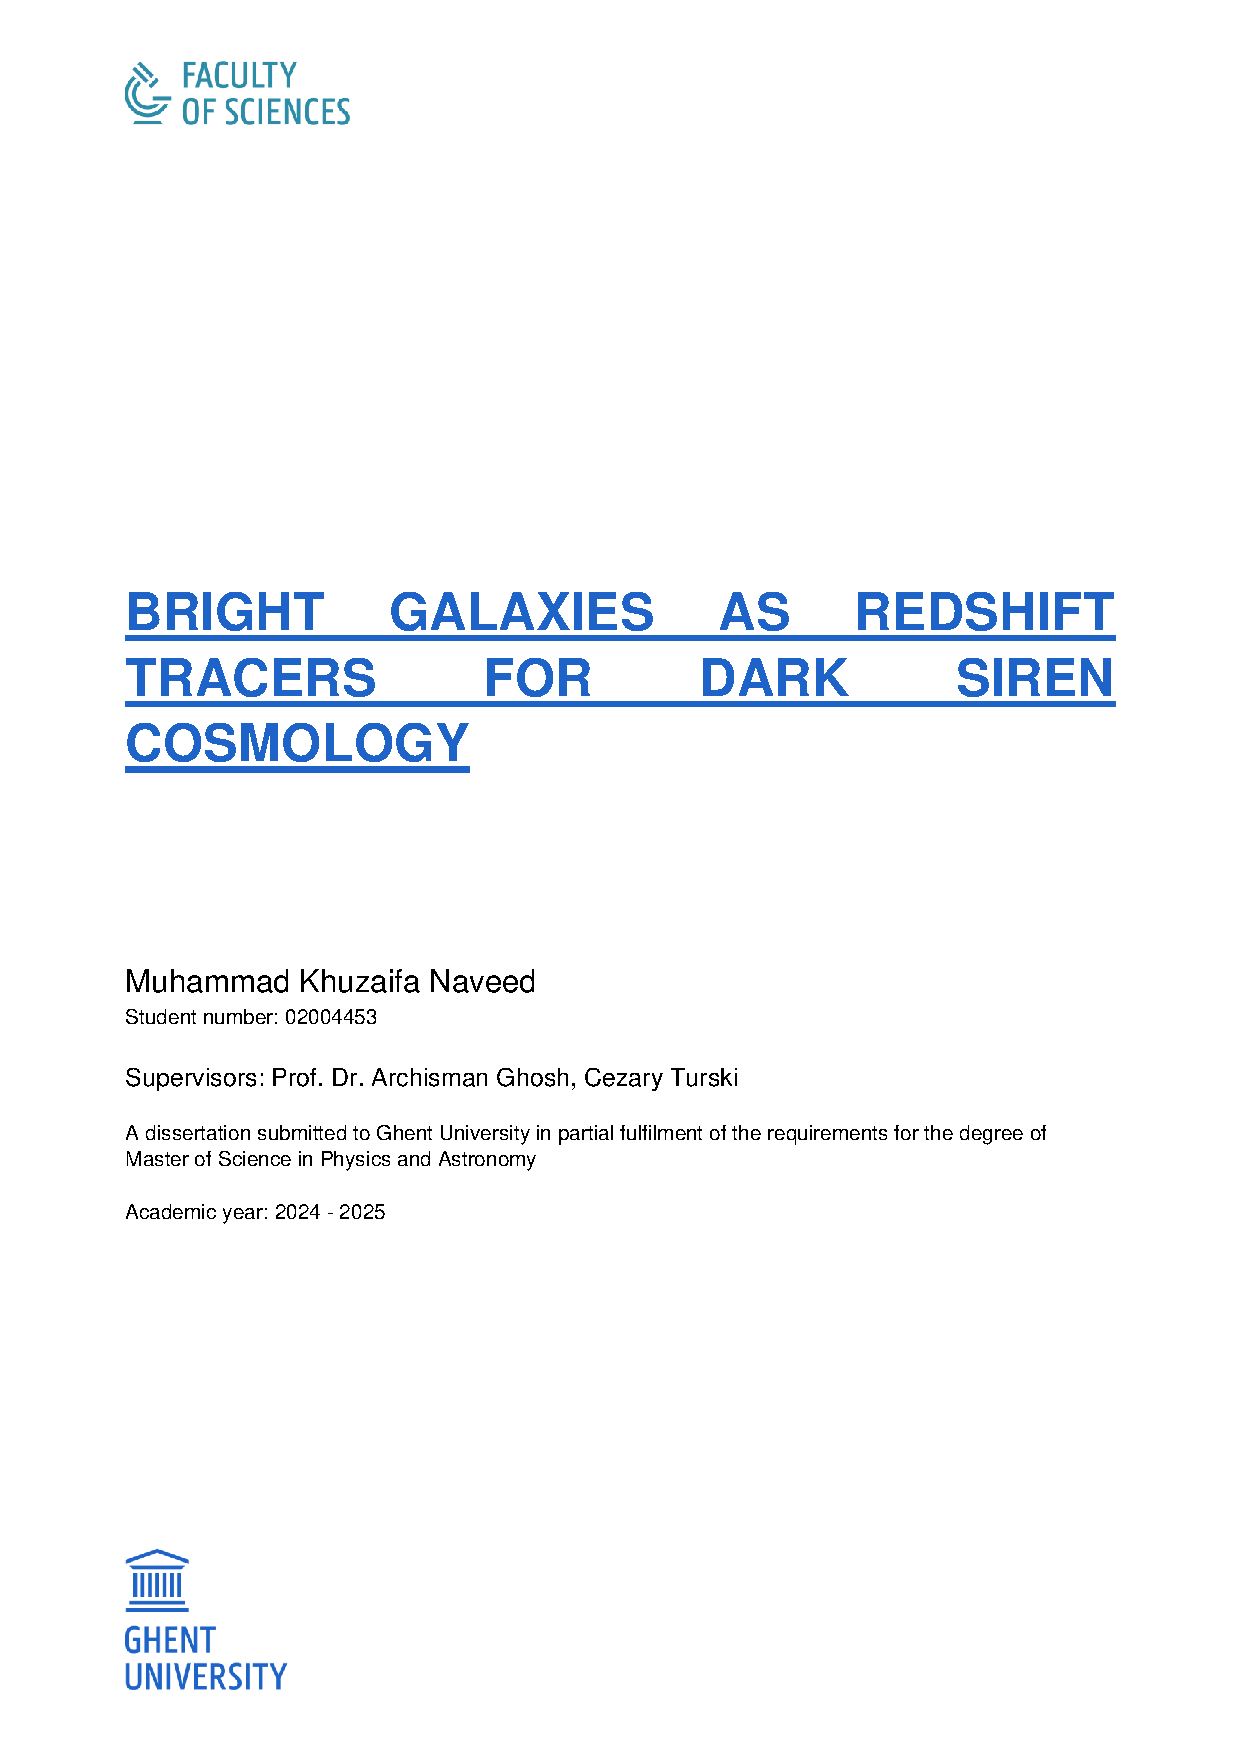
\includepdf[pages=-]{cover.pdf}

% ------------------------------------  --> main title page
\begin{titlepage}
	\pdfbookmark[0]{Titlepage}{Titlepage}
	\tgherosfont

	%{\Large \thesisUniversity} \\[4mm]
	
\includegraphics[width=3cm]{gfx/logo_ugent_en.png} \\[2mm]
	\textsf{\thesisUniversityDepartment} \\
	%\textsf{\thesisUniversityInstitute} \\
	\textsf{\thesisUniversityGroup} \\

	\vfill
	%{\large \thesisSubject} \\[5mm]
	{\LARGE \color{ctcolortitle}\textbf{\thesisTitle} \\[10mm]}
	{\Large \thesisName} \\

	\vfill
	%\begin{minipage}[t]{.27\textwidth}
	%	\raggedleft
	%	\textit{1. Reviewer}
	%\end{minipage}
	%\hspace*{15pt}
	%\begin{minipage}[t]{.65\textwidth}
	%	{\Large \thesisFirstReviewer} \\
	%  	{\small \thesisFirstReviewerDepartment} \\[-1mm]
	%	{\small \thesisFirstReviewerUniversity}
	%\end{minipage} \\[5mm]
	%\begin{minipage}[t]{.27\textwidth}
	%	\raggedleft
	%	\textit{2. Reviewer}
	%\end{minipage}
	%\hspace*{15pt}
	%\begin{minipage}[t]{.65\textwidth}
	%	{\Large \thesisSecondReviewer} \\
	%  	{\small \thesisSecondReviewerDepartment} \\[-1mm]
	%	{\small \thesisSecondReviewerUniversity}
	%\end{minipage} \\[10mm]
	\begin{minipage}[t]{.27\textwidth}
		\raggedleft
		\textit{Promotor} \\
		\textit{Day-to-day supervisor}
	\end{minipage}
	\hspace*{15pt}
	\begin{minipage}[t]{.65\textwidth}
		\thesisFirstSupervisor\\
		\thesisSecondSupervisor
	\end{minipage} \\[10mm]

	\thesisDate \\

\end{titlepage}


% ------------------------------------  --> lower title back for single page layout
\hfill
\vfill
{
	\small
	\textbf{\thesisName} \\
	\textit{\thesisTitle} \\
	\thesisSubject, \thesisDate \\
	%Reviewers: \thesisFirstReviewer\ and \thesisSecondReviewer \\
	Promotor: \thesisFirstSupervisor \\
	Day-to-day supervisor: \thesisSecondSupervisor \\[1.5em]
	\textbf{\thesisUniversity} \\
	\textit{\thesisUniversityGroup} \\
	%\thesisUniversityInstitute \\
	\thesisUniversityDepartment \\
	\thesisUniversityStreetAddress \\
	\thesisUniversityPostalCode\, \thesisUniversityCity
}
		% INCLUDE: all titlepages
\cleardoublepage

% !TEX root = ../thesis-example.tex
%
%************************************************
% Declaration
%************************************************
\pdfbookmark[0]{Declaration}{Declaration}
\chapter*{Declaration}
\label{sec:declaration}
\thispagestyle{empty}

You can put your declaration here, to declare that you have completed your work solely and only with the help of the references you mentioned.

\bigskip

\noindent\textit{\thesisUniversityCity, \thesisDateSubmission}

\smallskip

\begin{flushright}
	\begin{minipage}{5cm}
		\rule{\textwidth}{1pt}
		\centering\thesisName
	\end{minipage}
\end{flushright}

%*****************************************
%*****************************************

\clearpage
\newpage
\mbox{}

% !TEX root = ../thesis-example.tex
%
\pdfbookmark[0]{Acknowledgement}{Acknowledgement}
\chapter*{Acknowledgement}
\label{sec:acknowledgement}
\vspace*{-10mm}
%First and foremost, I would like to express my sincere gratitude to my promotor, Prof. Dr. Archisman Ghosh, for his guidance, support, and insightful feedback throughout this project. I am especially thankful for his flexibility and willingness to accommodate my schedule, which enabled me to work effectively under my own constraints. I am particularly grateful to my day-to-day supervisor, Cezary Turski, whose mentorship, patience, and consistent encouragement were instrumental throughout every phase of this thesis. His feedback, technical guidance, and responsiveness were key in helping me navigate both conceptual challenges and practical implementation. I deeply appreciate the time and effort they invested in my progress, and their understanding in adjusting to my working rhythm.
%
%I am also thankful to the GWCats collaboration for providing a valuable forum of expertise and exchange that informed several aspects of this research. A special thanks goes to Prof. Marcelle Soares-Santos for her early advice and for introducing me to the \texttt{BUZZARD} mock catalog, which shaped an important part of this thesis.
%
%I gratefully acknowledge the use of computational resources provided by the LIGO Laboratory computing clusters, which enabled the analysis performed in this work. Special appreciation is due to the developers and maintainers of the \texttt{gwcosmo} pipeline, the \texttt{GWSim} package, and the galaxy catalogs used in this work, including \texttt{GLADE+} and \texttt{BUZZARD}, whose open resources made this research possible.
%
%On a personal note, I am deeply grateful to my family for their unwavering support. In particular, I would like to thank my parents, whose love, encouragement, and sacrifices have made all of this possible. I am especially thankful to my mother, whose genuine interest in my work, despite having no background in the field, has always meant a great deal to me. Their belief in me has been the foundation of my academic journey, and I dedicate this work to them with immense gratitude. I also like to thank my friends for their timely distractions and unwavering companionship, which served as crucial reminders that there is, in fact, life beyond academic jargon and late-night analyses.
%
%Finally, I would like to thank everyone who contributed, directly or indirectly, to the successful completion of this thesis. Your support has meant more than words can convey.
%
\vspace{2em}
\noindent Muhammad Khuzaifa Naveed
 % INCLUDE: acknowledgement
\cleardoublepage

\pagestyle{plain}				% display just page numbers
% !TEX root = ../thesis-example.tex
%
\pdfbookmark[0]{Abstract}{Abstract}
\chapter*{Abstract}
\label{sec:abstract}
\vspace*{-13mm}
Gravitational-wave (GW) observations have introduced a powerful, independent method to measure the Hubble constant, $H_0$, through the use of so-called \textit{standard sirens}. This thesis investigates the use of \textit{dark sirens}, GW events without electromagnetic counterparts, for cosmological inference. In particular, it explores whether selecting the brightest galaxies as redshift tracers can improve the redshift prior and enhance the precision of $H_0$ estimation. By focusing on the most luminous galaxies, we partially mitigate the effects of catalog incompleteness currently plaguing dark siren measurements, effectively extending the reach of the catalog for cosmological analysis. Using the \texttt{gwcosmo} inference pipeline and the \texttt{GLADE+} galaxy catalog, a series of brightness-ranked percentiles were tested on a subset of the GWTC-3 catalog. The results show that moderate pruning improves $H_0$ constraints, while aggressive cuts lead to information loss and potential bias. Simulated mock data challenges using the \texttt{BUZZARD} catalog support this approach and reveal a lower pruning threshold near 30\% of the brightest galaxies. This method enhances the utility of incomplete galaxy catalogs in dark siren cosmology and contributes to the broader effort to resolve the Hubble tension.\\
\\

{\usekomafont{chapter} Samenvatting}\label{sec:abstract-nl}\\

\vspace*{-2mm}
Zwaartekrachtgolven (GW) bieden een krachtig en onafhankelijk middel om de Hubbleconstante, $H_0$, te meten via de zogenaamde \textit{standaard-sirenes}. Deze scriptie onderzoekt het gebruik van \textit{donkere sirenes}, GW-waarnemingen zonder elektromagnetische tegenhangers, voor kosmologische inferentie. In het bijzonder wordt nagegaan of het selecteren van de helderste sterrenstelsels als roodverschuivingstracers de $z$-prior kan verbeteren en zo de precisie van de $H_0$-schatting kan verhogen. Door ons te richten op de lichtkrachtigste sterrenstelsels wordt de impact van de onvolledigheid van bestaande sterrenstelscatalogi, een bekende uitdaging bij analyses met donkere sirenes, gedeeltelijk gemitigeerd, waardoor de effectieve diepte van de catalogus toeneemt. Met behulp van de \texttt{gwcosmo}-pipeline en de \texttt{GLADE+}-catalogus werd een reeks helderheidspercentielen getest op een subset van de GWTC-3-catalogus. De resultaten tonen aan dat gematigde afkappingen leiden tot een scherpere $H_0$ schatting, terwijl agressieve afkappingen resulteren in informatiederving en mogelijke bias. Gesimuleerde Mock Data Challenges met de \texttt{BUZZARD}-catalogus ondersteunen deze aanpak en wijzen op een praktische ondergrens van ongeveer 30\% van de helderste sterrenstelsels. Deze methode vergroot de toepasbaarheid van onvolledige sterrenstelscatalogi in donkere sirene-kosmologie en levert een bijdrage aan de bredere inspanningen om de Hubble-spanning op te lossen.
		% INCLUDE: the abstracts
\cleardoublepage

\setcounter{tocdepth}{2}		% define depth of toc
\tableofcontents				% display table of contents
\cleardoublepage

\phantomsection
\addcontentsline{toc}{chapter}{\listfigurename}
\label{lof:toc}

\listoffigures
\cleardoublepage

\phantomsection
\addcontentsline{toc}{chapter}{\listtablename}
\label{lot:toc}

\listoftables
\cleardoublepage

\phantomsection
\addcontentsline{toc}{chapter}{List of Abbreviations}
{\setkomafont{chapter}{\thesischapterfont\huge\bfseries} % Match the chapter font
\chapter*{List of Abbreviations}}
\begin{acronym}[ADDGALS]\itemsep8.0pt
  \acro{ADDGALS}{Adding Density-Determined Galaxies to Lightcone Simulations}
  \acro{BAO}{Baryon Acoustic Oscillation}
  \acro{BBH}{binary black hole}
  \acro{BCG}{Brightest Cluster Galaxy}
  \acro{BNS}{binary neutron star}
  \acro{CBC}{compact binary coalescence}
  \acro{CMB}{cosmic microwave background}
  \acro{DES}{Dark Energy Survey}
  \acro{EM}{Electromagnetic}
  \acro{GR}{General Relativity}
  \acro{GW}{Gravitational-Wave}
  \acro{GWTC}{Gravitational-Wave Transient Catalog}
  \acro{HST}{Hubble Space Telescope}
  \acro{JWST}{James Webb Space Telescope}
  \acro{KDE}{kernel density estimation}
  \acro{LOS}{line-of-sight}
  \acro{LVK}{LIGO, Virgo, KAGRA}
  \acro{MDC}{Mock Data Challenge}
  \acro{MNRAS}{Monthly Notices of the Royal Astronomical Society}
  \acro{NSBH}{neutron star black hole}
  \acro{SDSS}{Sloan Digital Sky Survey}
  \acro{SH0ES}{Supernovae H0 for the Equation of State}
  \acro{SNe}{supernovae}
  \acro{SNe Ia}{Type Ia supernovae}
  \acro{SNR}{signal-to-noise ratio}
  \acro{TRGB}{Tip of the Red Giant Branch}
  \acro{WISE}{Wide-Field Infrared Survey Explorer}
\end{acronym}

\cleardoublepage

% --------------------------
% Body matter
% --------------------------
\pagenumbering{arabic}			% arabic page numbering
\setcounter{page}{1}			% set page counter
\pagestyle{maincontentstyle} 	% fancy header and footer

\chapter{Introduction}
\label{chap:introduction}

\section{The Hubble Constant}
The Hubble constant, denoted $H_0$, quantifies the present-day expansion rate of the Universe. An empirical relationship between galaxy redshift and distance was published by Edwin Hubble in 1929~\citep{hubble1929}, showing that galaxies recede from us at velocities proportional to their distances. A few years earlier, Georges Lemaître had independently derived a similar velocity-distance relation in 1927~\citep{lemaitre1927univers}, based on theoretical grounds using general relativity and available data. This linear relation, now known as Hubble's law, is expressed as:
\begin{align}
    v = H_0 d
\end{align}
where $v$ is the recession velocity and $d$ is the proper distance to the galaxy. This linear relationship forms the foundation of modern observational cosmology, and established the expanding Universe as a cornerstone of modern cosmology laying the foundation for the standard cosmological model. 


In modern terms, the Hubble constant also governs the shape of the luminosity distance-redshift relation and determines the age and size of the Universe. In a flat $\Lambda$CDM cosmology, the Hubble constant enters the luminosity distance formula as:
\begin{align}
    d_L(z) = \frac{c(1+z)}{H_0} \int_0^z \frac{dz'}{\sqrt{\Omega_m(1+z')^3 + \Omega_\Lambda}}.
\end{align}
Accurate measurements of $H_0$ are essential for understanding the expansion history of the Universe and for anchoring other cosmological parameters. However, different observational methods have yielded inconsistent values, leading to a discrepancy, what is now known as the \textit{Hubble tension}.

\subsection{Early $H_0$ Measurements}
The quest to measure the Hubble constant has a long history, beginning with Hubble's original work in the 1920s. The first estimates of $H_0$ were based on the apparent brightness of Cepheid variable stars in nearby galaxies, which were used as standard candles~\citep{hubble1929}. These early measurements were limited by the available technology and the uncertainties in distance measurements.

In the 1930s, Edwin Hubble and Milton Humason measured redshifts and estimated distances to additional galaxies at Mount Wilson Observatory. Their work led to an initial estimate of $H_0 \approx 500~km~s^{-1}~Mpc^{-1}$, significantly higher than current values~\citep{hubble1936realm}. The discrepancy was largely due to underestimating galaxy distances and misidentifying Cepheid populations.

Throughout the 1940s and 1950s, astronomers like Walter Baade and Fritz Zwicky introduced new distance indicators, such as the use of Population I and II stars, and proposed Type Ia supernovae as standard candles~\citep{Baade1952,Baade1944,zwicky1942frequency}. Baade's recalibration of Cepheid distances effectively halved Hubble's original value, leading to estimates closer to $H_0 \approx 250~km~s^{-1}~Mpc^{-1}$~\citep{Baade1952,Longair_2006}.

Later on, the advent of techniques such as surface brightness fluctuations and the discovery of quasars enabled distance measurements over greater cosmological scales. However, large discrepancies persisted, with estimates of $H_0$ ranging from $50$ to $100~km~s^{-1}~Mpc^{-1}$~\citep{sandage1958current,,de1972velocity,sandage1982steps,de1985tycho}.

With the advent of the 21st century and significant advancements in both space-based and ground-based observational capabilities, including high-resolution radio telescopes and precision optical instruments, two independent and fundamentally different methods for measuring the Hubble constant emerged. One approach relies on the cosmic distance ladder, anchored by Cepheid variables and Type Ia supernovae, while the other infers $H_0$ from early-Universe observations of the \ac{CMB}, interpreted through the standard $\Lambda$CDM cosmological model.

\section{Modern Cosmology and the Hubble Tension}
\subsection{Local measurements: Cosmic Distance Ladder}
The traditional approach to measuring $H_0$ is the \textit{cosmic distance ladder}, which combines a series of interconnected distance indicators. The ladder begins with geometric parallax for nearby stars, continues with Cepheid variable stars in more distant galaxies, and culminates in the use of \ac{SNe Ia} as standard candles at cosmological distances. Each rung of the ladder calibrates the next, enabling a distance-redshift relation that extends to hundreds of megaparsecs~\citep{freedman2001final,Riess:2019cxk,cosmicdistanceladder,riess2022comprehensive}.

The 1980s and 1990s saw significant advancements in distance measurement techniques, including the use of the \textit{\ac{HST}} and improved calibration methods. The introduction of the \ac{HST} in 1990 allowed for more precise measurements of Cepheid variables in nearby galaxies, leading to a more accurate determination of $H_0$. The \ac{HST} Key Project, led by Freedman et al., used Cepheids in host galaxies of Type Ia supernovae to derive a value of $H_0 = 72 \pm 8~km~s^{-1}~Mpc^{-1}$~\citep{freedman2001final}. This result significantly improved both the precision and reliability of local distance measurements.

The \ac{SH0ES} project, which built upon the \ac{HST} Key Project, further refined the measurement of $H_0$ using a larger sample of Cepheid-calibrated supernovae. Recently, in 2022, they reported a value of $H_0 = 73.30 \pm 1.04~km~s^{-1}~Mpc^{-1}$~\citep{riess2022comprehensive}. Recently, results from the \ac{JWST} have also emerged~\citep{freedman2024status}. These results, while consistent with previous measurements, but raises questions about the underlying physics of cosmic expansion.

While the cosmic distance ladder achieves high precision, it involves multiple sources of systematic uncertainty at each step including stellar evolution models, metallicity corrections, dust extinction, and supernova standardization, all of which must be carefully calibrated and validated.

\subsection{Indirect measurements: Cosmic Microwave Background}
The second approach to measuring $H_0$ relies on the \textit{\ac{CMB}} radiation, which provides a snapshot of the Universe at a much earlier time. The \ac{CMB} is a relic radiation from the hot, dense state of the early Universe, and its temperature fluctuations encode information about the density and expansion rate of the Universe.

By fitting the observed power spectrum to the standard $\Lambda$CDM model, one can infer a value of the Hubble constant indirectly. This method relies on model assumptions, especially the flatness of the Universe and the constancy of dark energy. While not a direct measurement, the \ac{CMB}-based value of $H_0$ is internally consistent and extremely precise.

The introduction of the \textit{Planck} satellite in 2009 provided a new avenue for measuring $H_0$ through observations of the \ac{CMB}. The \ac{CMB} measurements, combined with the standard $\Lambda$CDM model, yielded a value of $H_0 = 67.4.30 \pm 0.5~km~s^{-1}~Mpc^{-1}$~\citep{Planck:2018vyg}. This value was significantly lower than the local measurements obtained from Cepheid-calibrated supernovae, leading to the emergence of the so-called \textit{Hubble tension}.

\begin{figure}[h!]
    \centering
    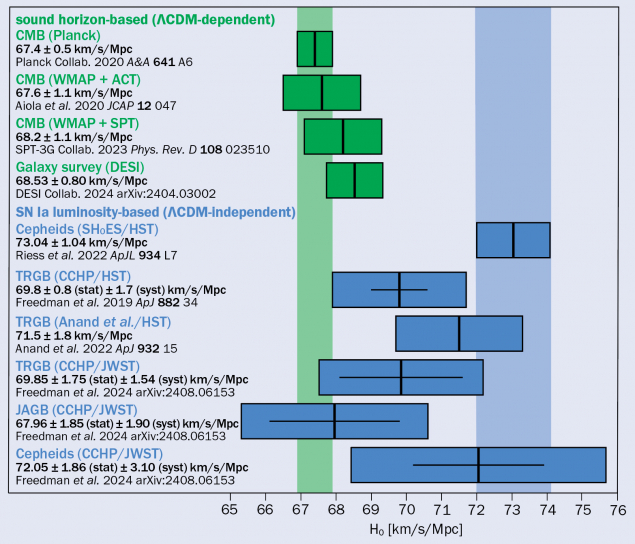
\includegraphics[width=0.9\textwidth]{figures/CCMarApr25_Hubble_tension.jpg}
    \caption[Comparison of local and \ac{CMB}-based measurements of Hubble constant.]{Hubble tension: Comparison of the local and \ac{CMB}-based measurements of $H_0$ over the years~\citep{cern2025}.}
    \label{fig:hubble_tension}
\end{figure}

\subsection{The Hubble Tension and quest for independent measurements}
The Hubble tension, now exceeding $5\sigma$, is one of the most significant unresolved issues in cosmology and has prompted investigations into both systematic errors and possible extensions to the standard cosmological model.
Independent methods are therefore crucial for arbitrating between these measurements. These include:
\begin{itemize}
    \item \textbf{\ac{TRGB}}\\
    The \ac{TRGB} method uses the well-defined luminosity at which low-mass stars ignite helium as a standard candle. This luminosity, shows minimal sensitivity to stellar population effects and dust, making it a robust alternative to Cepheid variables. The Carnegie-Chicago Hubble Program has applied this method to derive an independent calibration of Type Ia supernovae and obtained $H_0$ values closer to those inferred from the CMB~\citep{freedman2024status}. As such, \ac{TRGB} offers a valuable cross-check on the Cepheid-based ladder.
    \item \textbf{\ac{BAO}}\\
    \ac{BAO} are imprints of sound waves in the early Universe, visible as a characteristic scale in the clustering of galaxies. This scale acts as a standard ruler and allows geometric distance measurements across cosmic time. When combined with redshift data and a calibration from the sound horizon measured by the \ac{CMB}, \ac{BAO} can be used to infer $H_0$~\citep{cuceu2019baryon,alam2021completed}. Although \ac{BAO} are not purely local measurements, they offer a powerful, independent cosmological probe that is less susceptible to astrophysical systematics.

    \item \textbf{Gravitational-wave standard sirens}\\
    The use of gravitational-wave events as standard sirens provides a unique opportunity to measure $H_0$ independently.  The use of \ac{GW} sources as \textit{standard sirens}~\citep{schutz1986determining}, provide a direct measurement of the luminosity distance through their waveform. When combined with a redshift, obtained either via electromagnetic counterparts or galaxy catalogs, these events can trace the distance-redshift relation and yield an independent estimate of the Hubble constant.

    Standard sirens can be categoriezed into two broad categories: bright sirens and dark sirens, depending on whether an electromagnetic counterpart is detected. This thesis explores one implementation of this approach, focusing on \textit{dark sirens}: gravitational-wave events without identified electromagnetic counterparts. By statistically associating these events with potential host galaxies in wide-field catalogs, we aim to extract constraints on $H_0$. In particular, we investigate how restricting the galaxy catalog to its brightest subsets can improve the resulting cosmological inference.
\end{itemize}

Together, these emerging methodologies, TRGB, BAO, and standard sirens, form a triangulation of $H_0$ that spans distinct epochs and assumptions. Whether the Hubble tension reflects unknown systematics or fundamentally new physics, its resolution will likely come from the convergence (or divergence) of these independent measurements.

\begin{figure}[h!]
    \centering
    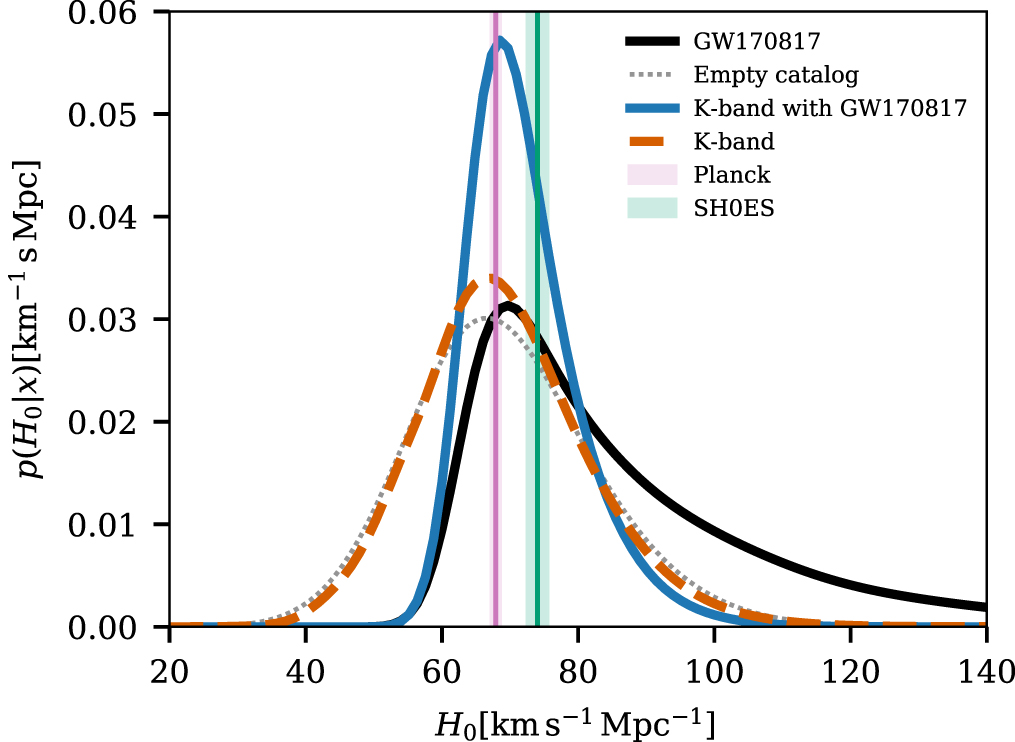
\includegraphics[width=0.8\textwidth]{figures/apjac74bbf9_hr.jpg}
    \caption[Hubble tension and standard sirens]{Hubble constant posterior from \ac{GWTC}-3 released by the \ac{LVK} collaboration, compared to the \ac{CMB} and local measurements. The tension between these measurements is evident, with the \ac{GW} posteriors (blue/orange), with/without the sole bright siren evenet, being consistent with both Planck (pink) and \ac{SH0ES} measurements, owing to the rather wide contraints. Additionally, the empty catalog (gray) and the bright siren (black) results are also plotted~\citep{abbott2023constraints}.}
    \label{fig:hubble_tension_gw}
\end{figure}


\section{\ac{GW} Cosmology}
\ac{GW} observations have introduced a novel, independent method for measuring cosmological distances: the so-called \textit{standard sirens}. First proposed by \citet{schutz1986determining}, standard sirens are the gravitational-wave analogs of \ac{EM} standard candles, such as Type Ia supernovae. Unlike \ac{EM} methods, standard sirens enable a direct, calibration-free determination of the luminosity distance from the observed waveform of a compact binary coalescence.

The amplitude and frequency evolution of the \ac{GW} signal encodes the luminosity distance, which can be inferred under the assumption of general relativity. However, \ac{GW} detectors are not sensitive to the redshift of the source. Therefore, to place a \ac{GW} event on the Hubble diagram and infer the Hubble constant $H_0$, one must independently obtain the redshift.

In the case of bright sirens, events with an \ac{EM} counterpart, such as GW170817~\citep{LIGOScientific:2017adf}, the redshift can be directly measured from the host galaxy spectrum. For the more common class of dark sirens, such as GW170814~\citep{DES:2019ccw}, where no \ac{EM} counterpart is detected, a statistical association is made between the \ac{GW} localization volume and galaxy catalogs. This association yields a redshift probability distribution, which can be combined with the luminosity distance posterior to constrain $H_0$.

The promise of standard sirens lies in their independence from traditional distance ladders and \ac{CMB} modeling. This makes them a crucial tool in addressing the Hubble tension. They are free from many astrophysical systematics affecting \ac{EM} methods, such as dust extinction, metallicity effects, or empirical calibrations. Additionally, because \acp{GW} are less susceptible to environmental interactions, they can probe larger cosmological volumes with fewer intermediate assumptions. As \ac{GW} detectors improve in sensitivity and the number of observed events increases, standard sirens are expected to play a progressively larger role in cosmological inference.

\section{Thesis Objectives}
The primary objective of this thesis is to investigate the impact of using brightness-ranked galaxy catalogs on the precision of $H_0$ measurements from dark sirens. By focusing on the brightest galaxies, we aim to improve the statistical constraints on $H_0$ while minimizing systematic uncertainties associated with galaxy catalog incompleteness.

This work involves $H_0$ inference using the \texttt{gwcosmo} pipeline, which combines \ac{GW} distance posteriors with galaxy redshift priors. We will explore the effects of applying brightness cuts to the galaxy catalog, examining how these cuts influence the resulting $H_0$ posterior distributions. The analysis will be performed on a subset of \ac{GWTC}-3 events, focusing on those with high \acp{SNR} and no known electromagnetic counterparts. The results will be validated through the use of simulated catalogs and mock data challenges, allowing us to assess the robustness of our findings.

In Chapter~\ref{chap:dark-siren-cosmology}, we will provide an overview of the theoretical framework for standard siren cosmology, including the principles of dark sirens. We will also discuss the challenges and limitations associated with this approach, particularly in the context of galaxy catalog incompleteness. Chapter~\ref{chap:data} details the data sources used in our analysis, including the \ac{GW} event catalog and galaxy catalogs. We will describe the selection criteria for the events and the modelling of missing \ac{EM} data. In Chapter~\ref{chap:methodology}, we will detail the methodology used in our analysis, including the construction of brightness-ranked galaxy catalogs and the statistical techniques employed to derive redshift priors. In particular the \texttt{gwcosmo} pipeline will be introduced, which combines the \ac{GW} distance posterior with the galaxy redshift prior to infer $H_0$. In this chapter we also present our results using real data and discusse the impact of brightness cuts on the resulting $H_0$ posterior distributions. In Chapter~\ref{chap:MDC}, we will present the results of our analysis using simulated catalogs and mock data challenges, allowing us to assess the robustness of our findings. Finally, in Chapter~\ref{chap:conclusion}, we will summarize our findings and discuss their implications for future research in cosmology.

\chapter{Gravitational-Wave Cosmology}
\label{chap:dark-siren-cosmology}

\section{Standard Siren Cosmology}

The detection of \acfp{GW} from \acp{CBC} have opened a transformative avenue in modern cosmology. These events acts as \textit{standard sirens}, the gravitational analog of standard candles, as the luminosity distance ($d_L$) to a \ac{GW} source is directly encoded in the strain amplitude and frequency evolution of the \ac{GW}. The amplitude, corrected for antenna pattern and inclination, provides a direct, calibration-free distance measurement under the assumption of general relativity.

From~\citet{maggiore2007gravitational}, the strain measured by a GW detector can be expressed as:
\begin{align}
h(t) = \frac{4}{d_L} \left( \frac{G\mathcal{M}_z}{c^2} \right)^{5/3}
       \left( \pi f(t) \right)^{2/3} F(\iota, \psi, \theta, \phi)
\label{eq:gw_strain}
\end{align}
where:
\vspace{-1em}
\begin{itemize}
    \item $h(t)$ is the strain measured at time $t$,
    \vspace{-1em}
    \item $d_L$ is the luminosity distance to the source,
    \vspace{-1em}
    \item $\mathcal{M}_z = (1+z)\mathcal{M}$ is the redshifted chirp mass,
    \vspace{-1em}
    \item $f(t)$ is the instantaneous GW frequency,
    \vspace{-1em}
    \item $F(\iota, \psi, \theta, \phi)$ is a function that captures the detector response depending on inclination angle $\iota$, polarization angle $\psi$, and sky position $(\theta, \phi)$.
\end{itemize}

The amplitude scaling with $1/d_L$ makes it possible to extract the luminosity distance directly from the signal, once the source's intrinsic properties and orientation are marginalized over. Furthermore, the $1/d_L$ scaling, in comparison to the $1/d_L^2$ scaling of \ac{EM} signals, means that \ac{GW} signals allow observations of sources at much larger distances, making them ideal for cosmological applications.

The direct self-calibrated measurement of the luminosity distance from the \ac{GW} signal is a key advantage of standard sirens over traditional \ac{EM} standard candles. This is in stark contrast to traditional \ac{EM} standard candles, such as \ac{SNe}, where the distance is inferred from the observed flux and requires a calibration step to account for the intrinsic brightness of the source. The \ac{GW} signal is also less affected by the intergalactic medium, as it is not subject to scattering or absorption like \ac{EM} signals. This allows for a more direct measurement of the distance to the source not affected by dust extinction or other astrophysical uncertainties that plague \ac{EM} observations. This makes \ac{GW} standard sirens a powerful tool for cosmology.

The concept of standard sirens was first introduced by Bernard F. Schutz, who noted that if the redshift of a \ac{GW} source can be measured, one could use \ac{GW} events to trace the  expansion history of the Universe, in particular an independent measurement of the Hubble constant ($H_0$) \citep{schutz1986determining}. This is due to the relation between the luminosity distance, redshift and the Hubble constant, in a flat \(\Lambda\)CDM cosmology, being:
\begin{align}
    d_L = \frac{c(1+z)}{H_0} \int_0^z \frac{dz'}{\sqrt{(1+z')^3\Omega_m + \Omega_\Lambda}}
\end{align}

Unlike traditional \ac{EM} methods, which require cross-calibration across multiple rungs of the distance ladder (parallax, Cepheids, SNe Ia) with each step introducing uncertainties that compound, the standard siren approach provides a direct cosmological probe. This reduces systematic uncertainties and provides an independent check on other $H_0$ measurement techniques, possibly providing a solution to the Hubble tension, the current discrepancy between local and global measurements of the Hubble constant \citep{Riess:2019cxk,Planck:2018vyg}.

However, a key limitation is that while \ac{GW} detectors provide a precise measurement of $d_L$, they do not directly measure the redshift. This necessitates an independent redshift measurement to place the source on the Hubble diagram. For \textit{bright sirens}, this redshift is obtained from the host galaxy identified via an \ac{EM} counterpart. In contrast, for \textit{dark sirens}, the redshift is inferred statistically by cross-referencing the \ac{GW} localization volume with galaxy catalogs or by leveraging population-based methods, as discussed in the following sections.

This forms the basis for \textit{standard siren cosmology}, where \ac{GW} sources are used as cosmic rulers. Over the past decade, this idea has transitioned from theoretical speculation to experimental reality, primarily through observations made by the \acf{LVK} collaboration. The first \ac{GW} event, \textbf{GW150914}, was detected in 2015, marking the beginning of a new era in astrophysics and cosmology \citep{abbott2016gw150914}. Since then, the \ac{LVK} collaboration has detected numerous \ac{GW} events, including \acf{BBH} mergers, \acf{BNS} mergers, and \acf{NSBH} mergers. These observations have provided valuable insights into the nature of gravity, the formation of compact objects, and the expansion history of the Universe.

\newpage
\section{Bright vs. Dark Sirens}
Standard sirens fall into two broad categories: \textit{bright sirens} and \textit{dark sirens}, depending on whether an electromagnetic counterpart is detected.

Bright sirens are rare but powerful. A prime example is \textbf{GW170817}, a \ac{BNS} merger detected by LIGO-Virgo in 2017, which was accompanied by a short gamma-ray burst and subsequent kilonova \citep{LIGOScientific:2017adf}. This multi-messenger event enabled the unambiguous identification of its \textit{host galaxy, NGC 4993}, providing both distance (from \ac{GW}) and redshift (from optical spectroscopy) measurements. The resulting Hubble constant measurement, $H_0 = 70.0^{+12.0}_{-8.0}~\mathrm{km}~\mathrm{s}^{-1}\mathrm{Mpc}^{-1}$, was a major milestone demonstrating that \ac{GW} observations could offer an independent and competitive cosmological probe \citep{LIGOScientific:2017adf}.

Such bright sirens provide a straightforward route to cosmological inference, using independent distance and redshift measurements. However, bright sirens require specific astrophysical conditions: the emission of \ac{EM} signals strong enough to be detected, accurate sky localization, and timely follow-up by optical telescopes. Such conditions are only met for a small fraction of \ac{CBC} events, especially those involving neutron stars. Majority of the observed mergers, especially \acfp{BBH} do not produce detectable \ac{EM} counterparts, and are thus classified as dark sirens.

In the absence of a direct redshift measurement, dark sirens require a \textit{statistical approach}. This involves cross-matching the sky localization and distance posterior from the \ac{GW} event with a galaxy catalog covering the relevant region. The redshift information of a number of candidate galaxies is then used to statistically infer the likely redshift distribution of the source. This is done by constructing a \textit{\acf{LOS} redshift prior} for each \ac{GW} event, which is then used to infer the Hubble constant. The LOS redshift prior is constructed by taking into account the galaxy number density and redshift distribution within the localization volume of the \ac{GW} event. The \ac{GW} localization volume is typically much larger than the volume of a galaxy, leading to a large number of galaxies that could potentially host the \ac{GW} event. This results in a large number of potential redshift measurements, which can be used to construct a more accurate \ac{LOS} redshift prior.

The statistical nature of dark sirens allows for the inclusion of a larger number of events, as it does not rely on the detection of an \ac{EM} counterpart. This is particularly important for \ac{BBH} events, which are more common and have a higher detection rate than \ac{BNS} events. 
%The \ac{LVK} collaboration has detected a large number of \ac{BBH} events, many of which are dark sirens. 
The \acf{LVK} collaboration has detected numerous dark siren events, which have been used to constrain the Hubble constant and test cosmological models~\citep{abbott2023constraints}.

As the number of \ac{BBH} detections increases with each observing run, dark sirens will dominate the future of standard siren cosmology. However, this statistical method introduces new complexities and depends heavily on the quality and completeness of the galaxy catalog used, which plays a pivotal role in the reliability of the inferred Hubble constant. The incompleteness of the galaxy catalog can lead to biases in the inferred redshift distribution, which can affect the accuracy of the Hubble constant measurement. This is particularly important for dark sirens, as they rely on the statistical association of \ac{GW} events with galaxies in the catalog. State of the art dark siren methods have been developed to mitigate these issues, but they still rely on the quality and completeness of the galaxy catalog used. The next section discusses the current state of the art in dark siren cosmology, including the challenges and limitations of existing methods.

\section{State of the Art Dark Siren Methods}
The statistical framework for dark siren cosmology has evolved rapidly. Early implementations relied on basic overlap between GW localization volumes and precompiled galaxy catalogs. The first generation of tools, including \texttt{gwcosmo}~\citep{gray2020cosmological, gray2022pixelated, gray2023joint} and \texttt{icarogw}~\citep{mastrogiovanni2021importance, mastrogiovanni2024icarogw}, introduced a more rigorous Bayesian framework: for each \ac{GW} event, a \textit{\ac{LOS} redshift prior} is constructed using galaxy number counts and redshifts, weighted by host probability, typically modeled using stellar mass proxies such as $K$-band luminosity.

One major challenge in this process is that current galaxy catalogs, such as \texttt{GLADE+} \citep{dalya2022glade+}, are incomplete beyond low redshift (typically $ z > 0.2 - 0.3$). This incompleteness leads to a nontrivial \textit{out-of-catalog} term in the redshift prior, which must be modeled analytically using a \textit{Schechter luminosity function}~\citep{gray2023joint, chen2024testing}. This function estimates the number density of missing faint galaxies, often assuming fixed parameters (e.g., $M_*,\alpha$) calibrated from deep surveys. If this modeling is inaccurate, the resulting posterior for $H_0$ can be biased or artificially broadened.

Despite these challenges, dark siren methods have been successfully applied to increasingly large datasets. The \ac{LVK} collaboration has published joint analyses using \ac{CBC} events from the \textbf{O1, O2,} and \textbf{O3} observing runs. For instance,~\citet{abbott2021gravitational, abbott2023constraints} presented cumulative constraints on $H_0$ using numerous \ac{CBC} events, demonstrating convergence toward a 10--15\% precision regime, albeit still limited by catalog systematics.

These analyses highlight the potential of dark sirens to provide competitive cosmological constraints, especially as galaxy catalogs improve and detection rates increase. Future observing runs, such as \textbf{O4} and \textbf{O5}, are expected to significantly enhance the statistical power of dark siren cosmology, potentially reducing uncertainties in $H_0$, providing better constraints on cosmological model, and testing the validity of general relativity on cosmological scales. The next generation of \ac{GW} detectors, such as the ground-based \textbf{Einstein Telescope}~\citep{Abac:ET} and \textbf{Cosmic Explorer}~\citep{Evans:CE}, and the space-based \textbf{LISA} observatory~\citep{LISA:2024hlh}, will further enhance the sensitivity and detection rates of \ac{GW} events, opening up new avenues for cosmological exploration.

\subsection{Redshift Inference Methods}
In dark siren cosmology, two principal strategies exist for inferring the redshift of gravitational-wave sources: the \textit{catalog-based method}~\citep{gray2020cosmological,gray2023joint,chen2024testing} and the \textit{population-based method}~\citep{ezquiaga2022spectral}. The catalog method, briefly discussed earlier, statistically associates \ac{GW} sources with galaxies from a survey by constructing a redshift prior along each line of sight, derived from galaxy positions and redshifts within the \ac{GW} localization volume. This approach captures the clustering of galaxies and allows for redshift inference when direct \ac{EM} counterparts are absent, but suffers from incompleteness at higher redshifts and spatial variation in survey depth~\citep{gray2020cosmological,gray2023joint,chen2024testing}. Conversely, the population method, often referred to as the \textit{spectral siren approach}, leverages features in the observed distribution of source-frame binary parameters, especially masses, which are redshifted in the detector frame. If the intrinsic mass distribution contains recognizable structure (e.g., a cutoff or peak), its displacement due to cosmic redshift can break the mass-redshift degeneracy, enabling cosmological inference independent of galaxy surveys~\citep{ezquiaga2022spectral}. However, this approach is sensitive to modeling assumptions about the underlying binary population. 

%If the intrinsic mass distribution contains recognizable structure (e.g., a cutoff or peak), its displacement due to cosmic redshift can break the mass-redshift degeneracy, enabling cosmological inference independent of galaxy surveys. In \ac{GW} observations, the detector-frame mass is related to the source-frame mass via $m_{\text{det}} = (1 + z)\, m_{\text{source}}$, making it difficult to disentangle intrinsic masses from redshift effects without external information~\citep{ezquiaga2022spectral, gray2023joint}. However, this approach is sensitive to modeling assumptions about the underlying binary population.
Recent work has sought to improve robustness by combining dark siren methods with \textit{spectral sirens}, extracting redshift information from the observed mass distribution of \ac{GW} sources under population synthesis assumptions~\citep{ezquiaga2022spectral}. These hybrid approaches aim to reduce dependence on incomplete catalogs and mitigate selection biases while extracting maximal cosmological information from current GW detections. Recently, both \texttt{gwcosmo} and \texttt{icarogw} have been updated to support such joint inference schemes~\citep{gray2023joint, mastrogiovanni2024icarogw}.

%Although powerful and refined, these methods are still limited by the incompleteness of the currently available galaxy catalog. This thesis aims to tackle this incompleteness problem, by refining the construction of the redshift prior. This is done by \textit{restricting the galaxy catalog to its brightest subset}, effectively making the catalog more complete. The rationale being that bright galaxies are better cataloged and more reliably associated with massive halos, which are more likely to host detectable GW events. By selectively using only the top $XX\%$ of galaxies by $K$-band luminosity, one can reduce the \textit{out-of-catalog contribution}, thereby increasing precision without strongly biasing the result. The upcoming chapters describe and validate this approach using real and mock data.

\subsection{Galaxy Weighting Choices}
In the construction of the \ac{LOS} redshift prior, each host galaxy is weighted by its probability of hosting a \ac{GW} event. This probability is typically modeled as a function of the galaxy's luminosity, and relies on the assumption that the merger host probability of a galaxy is related to its luminosity in a specific band. The choice of band remains uncertain, with different bands correlating with different aspects. The blue band, for instance, correlates with star formation rate and is therefore appropriate for mergers with short time delays (coalescence shortly after formation), while the near-infrared band correlates with the total luminous mass and is thus appropriate for mergers with longer time delays (mergers in older, more evolved galaxies). It is not known how exactly galaxy color is correlated with the merger rate.

\begin{figure}[ht]
    \centering
    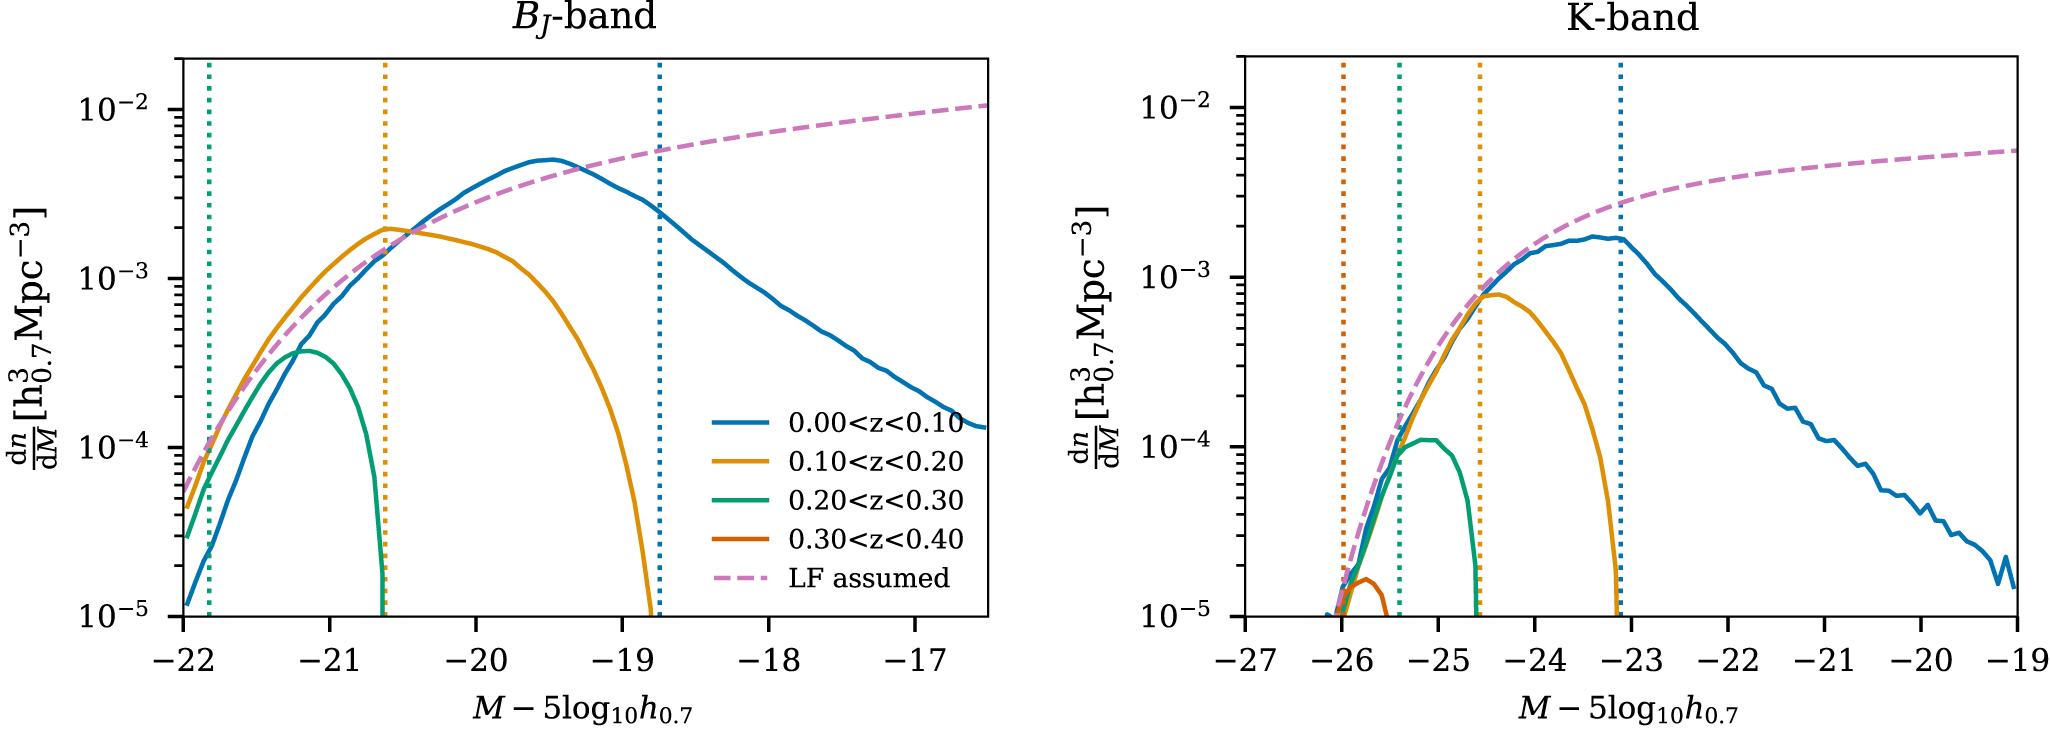
\includegraphics[width=\textwidth]{figures/apjac74bbf15_hr.jpg}
    \caption[The $B_J$-band and $K$-band luminosity function for the \texttt{GLADE+} catalog.]{The $B_J$-band (left) and $K$-band luminosity function (right) for the \texttt{GLADE+} catalog. The solid lines show the luminosity function of the catalog, while the dashed lines shows the assumed Schechter function. The vertical dashed line indicates the median absolute magnitude threshold for galaxy detection. The bright end of the $K$-band luminosity seems to match the assumed Schechter function, while the $B_J$-band luminosity function does not. This indicates that the assumption of a magnitude-limited catalog is not valid for the $B_J$-band~\citep{abbott2023constraints}.}
    \label{fig:luminosity_function}
\end{figure}

For modelling the out-of-catalog contribution, a Schechter luminosity function is assumed, which describes the distribution of galaxy luminosities in a given band. Wrong assumptions on the Schechter parameters, or incorrect description of selection biases can lead to biases in the inferred Hubble constant. The key assumption in constructing the out-of-catalog contribution is that the galaxy catalog is magnitude limited, i.e. galaxies are not detected only because they are too faint. If other selection biases (based on e.g., colors or spectral features) were present, the out-of-catalog contribution would be biased, leading to an incorrect estimate of the redshift prior \citep{abbott2023constraints}. 

If the assumption of a magnitude-limited catalog is valid, then the luminosity function of the galaxy catalog would match the assumed Schechter function at its bright end, and start to decrease as it reaches the corresponding absolute magnitude threshold. As can be seen in Figure~\ref{fig:luminosity_function}, this is indeed the case for the $K$-band luminosity function in \texttt{GLADE+}, which is well described by the assumed Schechter function. The $B_J$-band luminosity function, on the other hand, is not well described, and the assumption of a magnitude-limited catalog is not valid as there seem to be some additional missing galaxies at low redshift. This could lead to an incorrect estimate of the out-of-catalog contribution, and therefore an incorrect estimate of the redshift prior \citep{abbott2023constraints}. For this reason, traditionally, the $K$-band luminosity has been used for galaxy weighting in \ac{GW} cosmology inference pipelines. Another reason for using the $K$-band is, that the $K$-band luminosity is better correlated with the stellar mass of the galaxy, making it a more reliable tracer of the underlying matter distribution \citep{strazzullo2006near,sureshkumar2021galaxy,abbott2023constraints}. 

However, this choice is not without its limitations. The $K$-band luminosity is not always available for all galaxies in the catalog, leading to potential biases in the selection of galaxies used to construct the redshift prior. For example, the $K$-band luminosity is only available for about 1 million galaxies in the \texttt{GLADE+} catalog, which is a small fraction of the total number of galaxies in the catalog. This can lead to uncertainties in the redshift prior, which can in turn affect the inferred value of the Hubble constant. However, this effect should be relatively small, as we are interested in the overall matter distribution, and the $K$-band luminosity is a good tracer of the underlying matter distribution. This also forms the basis for this thesis, as we will be using the brightest galaxies in the $K$-band, in the \texttt{GLADE+} galaxy catalog, to trace the underlying matter distribution for improved $H_0$ inference as discussed in the next section.

\section{Refining the Redshift Prior: Brightest Galaxies as Tracers}
\begin{figure}[h!]
    \centering
    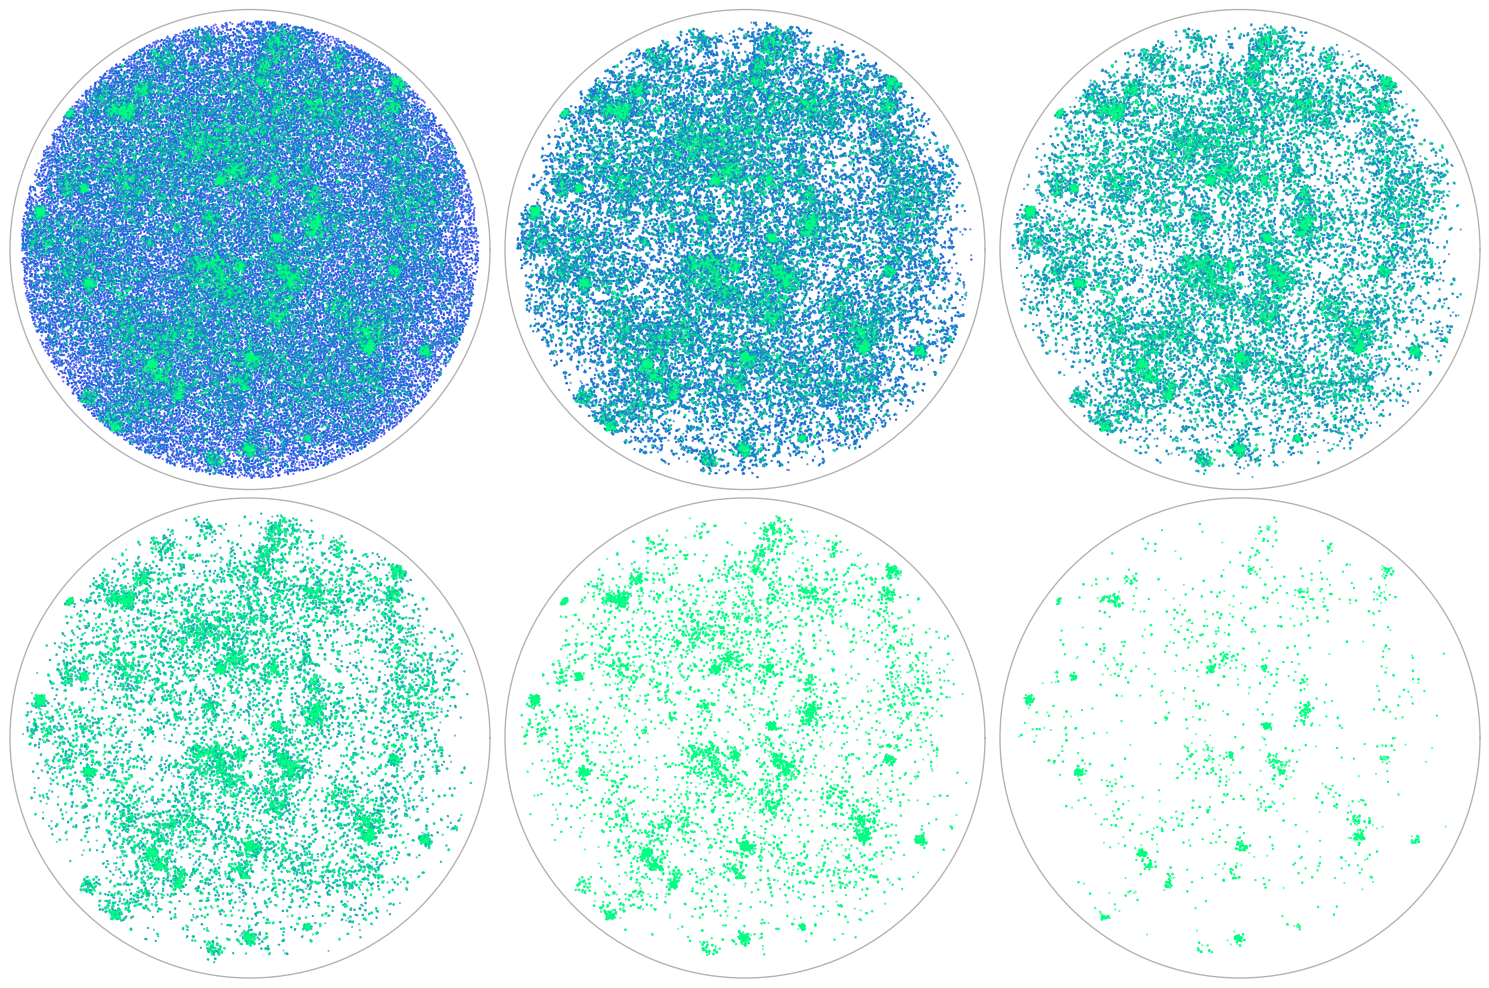
\includegraphics[width=\textwidth]{figures/depict7.png}
    \caption[Illustration of the proposed method, using bright galaxies as redshift tracers.]{Illustration of the proposed method for refining $H_0$ inference using the brightest galaxies as redshift tracers. The panels show different brightness cuts being applied to a galaxy catalog. The top left panel shows the case with a full galaxy catalog, while the subsequent panels (left-to-right) show the effect of applying increasingly strict brightness cuts. These depict how we can trace the matter distribution by using only the brightest galaxies. The last two panels (bottom center and right) show overly restrictive cuts, which would lead to a loss of information and a biased result. This is a conceptual visualization, generated with AI assistance, intended to represent the methodology rather than actual observational data.}
    \label{fig:depict}
\end{figure}

The current state of the art in dark siren cosmology relies heavily on the quality and completeness of the galaxy catalog used to construct the \ac{LOS} redshift prior. 
%The incompleteness of the galaxy catalog can lead to significant uncertainties in the redshift prior, which can in turn affect the inferred value of the Hubble constant. This is particularly important for dark sirens, as they rely on the statistical association of \ac{GW} events with galaxies in the catalog. 
The incompleteness of the galaxy catalog can lead to biases in the inferred redshift distribution, which can affect the accuracy of the Hubble constant measurement. State of the art dark siren methods have been developed to account for the incompleteness, but they still rely on the quality and completeness of the galaxy catalog used.

%While the statistical dark siren framework is powerful, its precision is ultimately limited by catalog incompleteness and the resulting need to model out-of-catalog galaxies. 
One strategy to mitigate this limitation is by refining the construction of the redshift prior by focusing on the \textit{brightest galaxies} to trace the underlying matter distribution. This would effectively make the catalog more complete and increase precision without introducing significant bias. The rationale is that the brightest galaxies are more likely to be associated with massive halos, which are in turn more likely to host detectable \ac{GW} events. The brightest galaxies are also more likely to be catalogued, as they are easier to detect and measure. These galaxies would also crudely trace the underlying matter distribution, since they are more likely to be associated with massive halos. This would be particulary useful for dark sirens, as they rely on the statistical association of \ac{GW} events with galaxies in the catalog. By replacing the redshift of the true host galaxy with the redshift of a nearby bright galaxy in the catalog, the small error incurred would be insignificant compared to the overall uncertainty in the redshift prior and the luminosity distance measurement.

Figure~\ref{fig:depict} illustrates this approach, highlighting how the brightest galaxies can be used to trace the underlying matter distribution. The last two panels in the figure show an overly restrictive cut, which would lead to a loss of information and a biased redshift prior. This emphasizes the importance of selecting an optimal brightness cut that balances the need for completeness with the desire for precision. The goal would be to find the optimal brightness cut that maximizes the precision of the redshift prior while minimizing bias.

This approach, of using the brightest galaxies to trace the matter distribution, is similar to the \textit{\ac{BCG}} method used in traditional cosmology, where the brightest galaxy in a cluster is used as a standard candle. The \ac{BCG} method has been shown to be effective in reducing the scatter in distance measurements and improving the precision of cosmological constraints \citep{lauer2014brightest}. By applying a similar approach to dark sirens, one can potentially improve the precision of the inferred Hubble constant without introducing significant bias.

To implement this approach, we define a subset of the \texttt{GLADE+} galaxy catalog, \texttt{GLADEPXX}, which includes only the top $XX\%$ of galaxies ranked by $K$-band luminosity, as the $K$-band luminosity is better associated with the mass of the galaxies \citep{strazzullo2006near,sureshkumar2021galaxy}. The construction of the LOS redshift prior is then modified to account for this restricted catalog. Specifically, the Schechter luminosity function is adjusted to reflect the brighter subset, making the out-of-catalog contribution smaller, effectively making the catalog more complete. This modified prior is then used in the Bayesian framework to infer the Hubble constant.

The next chapters provide a detailed description of the methodology, including the \texttt{gwcosmo} inference pipeline, the selection criteria for \texttt{GLADEPXX}, the modeling of the out-of-catalog part and the validation of this approach using mock data.
\chapter{Data}
\label{chap:data}


The foundation of any standard siren cosmological analysis lies in the quality, completeness, and coverage of the data. In this thesis, we rely on two primary data sources: \ac{GW} observations from the \acf{LVK} detectors, and galaxy catalogs providing \ac{EM} redshift information. These datasets are used in tandem to statistically contruct a redshift prior for each \ac{GW} event and ultimately to constrain the Hubble constant $H_0$.

\section{\ac{GW} Event Data}

\subsection{The GWTC-3 Catalog}

The \ac{GW} data used in this study are obtained from the \textit{\acf{GWTC}}~\citep{abbott201gwtc1, abbott2021gwtc2, abbott2023gwtc3, abbott2024gwtc21}. This catalog comprises all \ac{CBC} events detected during the three observing runs (O1, O2, and O3) of the Advanced LIGO and Virgo detectors. \ac{GWTC} includes over 93 confident detections, primarily \acf{BBH} mergers, along with a few \acf{NSBH} and \acf{BNS} systems.

For each event, the catalog provides posterior samples for key source parameters inferred through Bayesian parameter estimation. These include the detector-frame component masses $(m_{1}^{\text{det}}, m_{2}^{\text{det}})$, the luminosity distance $d_L$, sky location (right ascension $\alpha$ and declination $\delta$), orbital inclination angle $\iota$, chirp mass $\mathcal{M}$, and various spin parameters (e.g., $\chi_{\text{eff}}$, $\chi_1$, $\chi_2$). These samples form the basis for constructing the luminosity distance posterior and are essential inputs to the standard siren inference pipeline.

%\subsection{Evant Parameter Estimation?}
%Is it needed to mention the parameter estimation? I think not.
%
\subsection{Event Selection Criteria}

To focus our analysis on dark siren cosmology, we restrict our sample to events that do not have any confirmed electromagnetic counterpart (i.e., no associated kilonova or GRB), have a network \ac{SNR} exceeding 11, have somewhat good sky localization, and are accompanied by publicly available posterior samples for distance and sky position.

These criteria are designed to ensure both the statistical robustness of the inference and compatibility with existing galaxy catalogs. After applying these cuts, a subset of 47 events, with 42 \acp{BBH}, 3
\acp{NSBH}, and 2 \acp{BNS}, is retained for cosmological analysis.

\subsection{Distance Posteriors and Sky Localization}

Each event is characterized by a posterior distribution over the three-dimensional localization volume, typically encoded using the HEALPix format. The posterior provides the probability density $p(d_L, \alpha, \delta)$, where $d_L$ is the luminosity distance and $(\alpha, \delta)$ denote right ascension and declination.

These distance posteriors are crucial for constructing the \ac{LOS} redshift prior when cross-matched with galaxy catalogs. Events with poor localization or multimodal distance distributions contribute more uncertainty to the inferred $H_0$, emphasizing the importance of event quality.

\subsection{Assumptions About the Source Population}
\label{sec:source_population}

Although this thesis primarily focuses on statistical redshift modeling, it is important to acknowledge that the cosmological inference also depends weakly on assumptions about the source population. For instance, \texttt{gwcosmo} allows one to specify priors on:
\begin{itemize}
  \item Merger rate evolution with redshift, typically modeled as \( R(z) \propto (1+z)^\kappa \)
  \vspace{-1em}
  \item Mass distributions of the binaries
\end{itemize}

For our analysis we assume that \acp{CBC} follow a Madau-Dickinson merger redshift evolution model \citep{madau2014cosmic}:
\begin{align}
    R(z) = R_0(1+z)^{\gamma}\frac{1+(1+z_p)^{-(\gamma+\kappa)}}{1+\left( \frac{1+z}{1+z_p}\right)^{\gamma + \kappa}}
\end{align}
Here $R_0$ is the local merger rate, $\kappa$ the high-z slope, $\gamma$ the low-z slop and $z_p$ the break-point. All the assumed priors, taken from \citet{abbott2023gwtc}, are given in Table \ref{tab:Madau}.

For \ac{BBH} we use power-law with a Gaussian peak mass model, with powerlaw slope $\alpha$, the mean of the Gaussian $\sigma_g$, the width 
of the peak $\mu_g$, and the relative weight between power-law and
the peak $\lambda_g$. We also assume the minimum and maximum masses for the black hole distribution. For neutron stars we assume that
mass is uniformly distributed between $M_{min,NS}$ and
$M_{max,NS}$. All the assumed priors, taken from \citet{abbott2023gwtc}, are given in Table \ref{tab:mass_dist}.

\begin{table}[h!]
    \small
    \centering
    \caption{Priors on merger rate shape parameters.}
    \label{tab:Madau}
    \begin{tabular}{c l}
        \hline
        \textbf{Parameter} & \textbf{Prior} \\
        \hline
         $R_0$ & $1/R_0$ (implicit) \\
         $\kappa$ & $2.86$ \\
         $\gamma$ & $4.59$ \\
         $z_p$ & $2.47$ \\
         \hline
    \end{tabular}
\end{table}

\begin{table}[h!]
    \small
    \centering
    \caption{Priors on the mass model parameters.}
    \label{tab:mass_dist}
    \begin{tabular}{c l}
        \hline
        \textbf{Parameter} & \textbf{Prior} \\
        \hline
         $\alpha$ & $3.78$ \\
         $\sigma_g$ & $3.88$ \\
         $\mu_g$ & $32.27$ \\
         $\lambda_g$ & $0.03$ \\
         $M_{min,BH}$ & $4.98M_{\odot}$ \\
         $M_{max,BH}$ & $112.5M_{\odot}$ \\
         $M_{min, NS}$ & $1.0M_{\odot}$ \\
         $M_{max, NS}$ & $3.0M_{\odot}$ \\
         \hline
    \end{tabular}
\end{table}

\newpage

\section{\ac{EM} Galaxy Catalogs}

\subsection{The \texttt{GLADE+} Galaxy Catalog}

For redshift information, we use the \texttt{GLADE+} galaxy catalog~\citep{dalya2022glade+}, an extended version of the original \texttt{GLADE} catalog~\citep{dalya2018glade}, designed for \ac{GW} follow-up. \texttt{GLADE+} is a composite catalog that combines several large surveys to achieve all-sky coverage:
\vspace{-1em}
\begin{itemize}
  \item 2MASS XSC and 2MPZ: infrared-based all-sky surveys~\citep{skrutskie2006two, bilicki2013two} 
  \vspace{-1em}
  \item WISExSCOS: photometric redshifts from the \ac{WISE} and the SuperCOSMOS survey~\citep{bilicki2016wise}
  \vspace{-1em}
  \item HyperLEDA: spectroscopic redshift survey~\citep{makarov2014hyperleda}
  \vspace{-1em}
  \item SDSS DR16Q: quasar catalog~\citep{lyke2020sloan}
\end{itemize}

As of the latest release, \texttt{GLADE+} includes over 22 million objects with available positions, redshifts (spectroscopic or photometric), and photometry in multiple bands, most critically the $K$-band~\citep{dalya2022glade+}.

\subsection{Catalog Completeness}
\label{sec:luminosity_function}

A significant limitation of \texttt{GLADE+} is its incompleteness beyond redshift $z \sim 0.3$. While the catalog is approximately complete for bright galaxies at low redshift, its coverage of fainter galaxies or more distant regions is limited. This incompleteness introduces a bias when performing statistical redshift inference, as missing galaxies contribute to the out-of-catalog part of the redshift prior.

To address this, the \texttt{gwcosmo} pipeline models the galaxy population, for the out-of-catalog region, using a truncated Schechter luminosity function:
\begin{align}
    \phi(M) \propto 10^{0.4(\alpha + 1)(M - M^*)} \exp[-10^{0.4(M - M^*)}]
\end{align}
where \( M \) is the absolute magnitude in the $K$-band, $M^*$ is the characteristic magnitude, and $\alpha$ is the faint-end slope. For our analysis, we adopt the standard parameters: $\alpha = -1.09$, $M^*_K = -23.39 + 5\log h$, consistent with \citet{kochanek2001k}, and truncate at $M^*_{K,min} = -27.00 + 5\log h$ and $M^*_{K,max} = -19.00 + 5\log h$.

\subsection{Redshift Uncertainty Modeling}

Redshift measurements in \texttt{GLADE+} are heterogeneous. Spectroscopic redshifts are generally precise, but photometric redshifts can have uncertainties on the order of $\sigma_z \sim 0.01-0.05$. These uncertainties are modeled by convolving the redshift of each galaxy with a Gaussian of fixed width, an assumption used in constructing the redshift prior.

Additionally, to reduce systematic error, galaxies with unphysical redshifts or unreliable photometry are filtered out during preprocessing. The net result is a cleaned, sky-localized, and redshift-tagged galaxy distribution that can be used for \ac{LOS} prior construction.

Furthermore, $K$-corrections are applied in \texttt{gwcosmo} following \citet{kochanek2001k}, and the apparent magnitude thresholds $m_{thr}$ are computed per HEALPix pixel as a median apparent magnitude in a given pixel, giving a $K$-band threshold of 13.5 on average.

\subsection{$K$-band Luminosity as Host Probability Proxy}

In dark siren analysis, we must assign each galaxy a probability of being the true host. Following common practice, this probability is assumed to scale with stellar mass, for which $K$-band luminosity serves as a good proxy~\citep{strazzullo2006near,sureshkumar2021galaxy}. The host probability  $p_i$ for each galaxy is given by:
\begin{align}
    p_i \propto L_{K, i}
\end{align}
This choice is motivated by the assumption that more massive galaxies are more likely to host \acp{CBC} events. While simplistic, it provides a reasonable baseline.
\chapter{GLADE+ Bright Galaxies as Redshift Tracers}
\label{chap:methodology}

The core idea investigated in this thesis is the use of \textbf{bright galaxies} as redshift tracers for \ac{GW} events. The \texttt{GLADE+} galaxy catalog is a comprehensive database of galaxies in the local universe, but it suffers from incompleteness at high redshifts. This incompleteness arises from the limited depth of the catalog, which is primarily designed to cover the local universe, owing to the sensitivity constraints of the current \ac{EM} telescope. We overcome this limitation by focusing on the brightest galaxies in the catalog, which are more likely to be well-represented and can provide a more accurate estimate of the redshift of \ac{GW} events. This essentiaally makes the catalog deeper and more complete at high redshifts, while allowing us to use the \texttt{GLADE+} catalog as a proxy for the underlying matter distribution in the universe.


\section{Bright Galaxy Subsets}
The analysis begins with the construction of \textbf{bright galaxy subsets}, denoted \texttt{GLADEPXX}, where only the top $XX\%$ of galaxies by cumulative $K$-band luminosity are included. The $K$-band luminosity is chosen as it is better associated with the mass of the galaxies \citep{strazzullo2006near,sureshkumar2021galaxy}. Limiting the analysis to these bright subsets allows us to:
\vspace{-1em}
\begin{itemize}
  \item Reduce the out-of-catalog correction by focusing on galaxies likely to be well-represented.
  \vspace{-1em}
  \item Improve the signal-to-noise ratio of the statistical redshift prior.
  \vspace{-1em}
  \item Minimize the inclusion of poorly characterized or faint galaxies.
\end{itemize}

The bright galaxy subsets are defined by selecting galaxies based on their absolute magnitude, which is inferred from their redshift and apparent magnitude. For a given subset, the dimmest galaxy sets the absolute magnitude limit, $M_{max}$, for that subset. This limit is then used in the Schechter luminosity function to adjust the out-of-catalog contribution, effectively reducing its impact. By focusing on the brightest galaxies, we assume that they trace the mass distribution in the Universe more effectively, and are more likely to host \ac{CBC} events.

This approach improves the completeness of the galaxy catalog in the high-redshift regime, as the out-of-catalog contribution becomes smaller. Figure~\ref{fig:z_dist} illustrates how the redshift distribution shift towards higher values making the catalog more complete, highlighting the effectiveness of this method in probing deeper $z$--ranges.

\begin{figure}[h!]
  \centering
  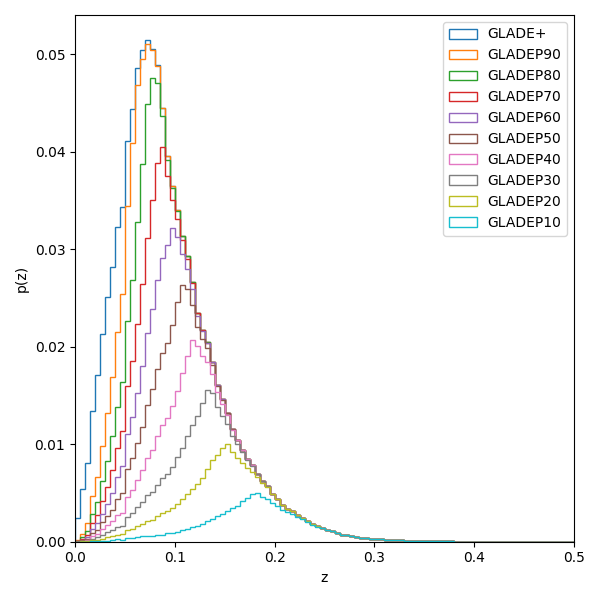
\includegraphics[width=0.7\linewidth]{figures/z_dist_perc.png}
  \caption[Normalized redshift distributions $p(z)$ for the GLADE+ galaxy catalogue and the brightest percentiles.]{Normalized redshift distributions $p(z)$ for the full GLADE+ galaxy catalogue (blue) and the brightest percentiles (other curves). Each subset, labeled “GLADEPXX,” includes only the top XX\% brightest galaxies in the $K$-band. Focusing on increasingly brighter subsets shifts and sharpens the redshift distribution, effectively probing deeper ranges in $z$.}
  \label{fig:z_dist}
\end{figure}

\subsection{Trade-Offs and Limitations}

While bright subsets reduce catalog incompleteness, they may inadvertently exclude genuine host galaxies, especially if those lie in less luminous systems or in underrepresented regions of the catalog. The effectiveness of these cuts depends on the intrinsic distribution of host galaxies, the depth and completeness of the original catalog, and the accuracy of $K$-band photometry. 
%The effectiveness of these cuts therefore depends on:
%\vspace{-1em}
%\begin{itemize}
%  \item The depth and completeness of the original catalog.
%  \vspace{-1em}
%  \item The intrinsic distribution of host galaxies.
%  \vspace{-1em}
%  \item The accuracy of $K$-band photometry.
%\end{itemize}

One major limitation of this approach is that brightest galaxies may not be representative of the overall galaxy population, as they may be biased towards certain types of galaxies or regions of the sky. This effect is however mitigated by the fact that we are using the $K$-band luminosities, which are good tracer for the stellar mass \citep{strazzullo2006near,sureshkumar2021galaxy}, and in turn the overall matter distribution. Furthermore, the bright galaxy subsets are constructed from the \texttt{GLADE+} catalog, which is designed to be a complete and representative sample of galaxies in the local universe. This means that the bright galaxy subsets are likely to be representative of the overall galaxy population, and give a crude estimate of the matter distribution, even if they are not a complete sample.

Estimating the true redshift of a \ac{GW} event by the nearest brightest galaxies is supposed to have a negligible effect on the results. This is because the bright galaxies are more likely to be located in regions of high density, such as galaxy clusters or groups, which are also likely to host \ac{GW} events. This means that the bright galaxies are likely to be located in the same large-scale structure as the \ac{GW} event, and thus provide a good estimate of the redshift of the event. 

One important thing to note is that while the use of a bright subset enhances the completeness of the catalogue at high redshifts, it also introduces a trade-off. If the brightness cut is too restrictive, the exclusion of fainter galaxies may lead to an underrepresentation of the overall matter distribution, potentially biasing the results. One needs to carefully balance these considerations by comparing different brightness thresholds. A moderate brightness cut will maximize the benefit in terms of depth without incurring significant bias.

The appropriate brightness cut can be established only via a set of astrophysics-motivated large-scale simulations. A \ac{GW} \textit{\ac{MDC}} using the simulated \texttt{BUZZARD} galaxy catalog from the \ac{DES} Collaboration~\citep{DES:2019jmj,DES:2021bwg}. It is designed to determine the optimal brightness threshold which maximizes the measurement precision with bright subsets while keeping the biases in control. Tests performed in the process will help refine the methodology and ensure that the improved constraints on the Hubble constant are robust against additional systematic uncertainties.

While the bright galaxy subsets may not be a perfect representation of the overall galaxy population, they are still a useful tool for improving the completeness of the galaxy catalog and reducing the out-of-catalog correction. The error incurred by using the bright galaxies as redhsift tracers maybe small compared to the current errors in luminosity distance measurements from the \ac{GW} events, this may become a problem in the future as the \ac{GW} measurements become more precise. In this case, one may need to use more sophisticated methods to estimate the redshift of the \ac{GW} event, such as more complex models of the galaxy population, but for now this is a good first step towards improving the completeness of the galaxy catalog and reducing the out-of-catalog correction, by leveraging the currently available \ac{EM} data.

%In Chapters~\ref{chap:results} and~\ref{chap:mockdata}, we quantify these trade-offs using both real data and mock catalogs.

\section{The \texttt{gwcosmo} Pipeline}
Based on the work presented in \cite{gray2020cosmological,gray2022pixelated,gray2023joint}, \texttt{gwcosmo} is a Python package specifically designed for the joint inference of cosmological parameters using data from standard sirens and galaxy catalogs.  The pipeline employs Bayesian inference techniques to simultaneously constrain cosmological parameters, such as the Hubble constant and dark energy equation of state parameters. It does this using various data inputs, including the gravitational wave strain data from gravitational wave observatories such as LIGO, Virgo, and KAGRA, entries from galaxy catalogs containing photometric or spectroscopic redshift information, as well as other relevant galaxy properties, and \ac{CBC} source population models. 

\texttt{gwcosmo} represents a significant advancement in extracting cosmological information especially from \ac{CBC} events that lack unique \ac{EM} counterparts. It addresses the challenge of redshift inference in dark siren cosmology by statistically marginalizing over potential host galaxies from a flux-limited catalog. This is achieved through hierarchical Bayesian modeling that incorporates \ac{GW} strain data, the spatial and redshift distribution of galaxies, and astrophysical population models.

The pipeline is designed to be flexible and extensible, allowing users to customize the models and priors used in the analysis. It also provides tools for visualizing the results, including posterior distributions and confidence intervals for the inferred parameters. The package is built on top of established libraries such as \texttt{numpy}, \texttt{scipy}, and \texttt{matplotlib}, making it accessible to researchers familiar with these tools.
The \texttt{gwcosmo} pipeline is a particularly useful tool in the intersection of gravitational wave astronomy and cosmology, as it enables the extraction of valuable cosmological information from gravitational wave events, which can complement traditional methods of measuring cosmological parameters. The package is actively maintained and updated to incorporate new developments in both gravitational wave detection and cosmological modeling, ensuring that it remains a relevant tool for researchers in the field.

\subsection{Bayesian Framework: \textbf{TO BE UPDATED}}
The goal is to evaluate the posterior distribution:
\begin{equation}
p(\Lambda \mid \{d_{\text{GW}}\}, \{d_{\text{EM}}\}) \propto p(\Lambda) \, p(\{d_{\text{GW}}\}, \{d_{\text{EM}}\} \mid \Lambda),
\end{equation}
where:
\begin{itemize}
  \vspace{-1em}
  \item $\Lambda$ are the hyperparameters of interest (e.g., cosmological parameters, population hyperparameters),
  \vspace{-1em}
  \item $d_{\text{GW}}$ are the GW observables (e.g., luminosity distance posteriors),
  \vspace{-1em}
  \item $d_{\text{EM}}$ are the galaxy catalogue data (e.g., redshifts, magnitudes, positions).
\end{itemize}

The likelihood is approximated by marginalizing over all galaxies $k$ within the GW localization volume:
\begin{equation}
p(\Lambda \mid \{d_{\text{GW}}\}, \{d_{\text{EM}}\}) \propto \prod_{i} \sum_{k} w_k \, p(d_{\text{GW},i} \mid z_k, \Lambda),
\end{equation}
where $w_k$ is the weight assigned to each galaxy, typically modeled based on a proxy for host probability (e.g., luminosity in a selected band, merger rate evolution).

\subsection{Key Features of \texttt{gwcosmo}}
Some of the key features of the \texttt{gwcosmo} pipeline include:
\begin{itemize}
  \item \textbf{Joint Population + Cosmology Inference:} Simultaneously samples over cosmological parameters and population hyperparameters, avoiding bias from fixed population assumptions.
  \item \textbf{Galaxy Catalogue Weighting:} Utilizes \ac{LOS} redshift priors constructed from galaxy distributions, incorporating completeness corrections based on flux thresholds.
  \item \textbf{Selection Effects:} Corrects for GW detector sensitivity and incompleteness in galaxy catalogues by modeling detection probabilities and magnitude limits.
\end{itemize}

\subsection{Implementation and Applications}

The pipeline is implemented in Python and uses \ac{KDE} of \ac{GW} posteriors and efficient catalog summation to handle discrete and incomplete galaxy data. The most recent version was applied by \cite{gray2023joint} to reanalyze 47 events from the \ac{GWTC}-3 catalog using the \texttt{GLADE+} galaxy catalog, yielding an updated measurement of the Hubble constant:
$$
H_0 = 69^{+12}_{-7}~\text{km s}^{-1}~\text{Mpc}^{-1}.
$$

\texttt{gwcosmo} is publicly available and is expected to be a useful tool for future gravitational-wave cosmology with upcoming detector runs and deeper galaxy surveys.

\section{\ac{LOS} Redshift Prior}
We base our analysis on the \texttt{gwcosmo} pipeline \citep{gray2020cosmological,gray2022pixelated,gray2023joint}, which relies on a precomputed \ac{LOS} redshift prior, a prior on the \ac{GW} signal's redshift and direction. This \ac{LOS} redshift prior is used in tandem with the luminosity distance posterior from the \ac{GW} signal, to get a measurement for the Hubble constant $H_0$.

\subsection{\ac{LOS} Redshift Prior Construction}
The \ac{LOS} redshift prior is constructed from the \texttt{GLADE+} galaxy catalog, which contains a wealth of information about the galaxies in the local universe. The redshift prior is constructed by taking into account the distribution of galaxies along the line of sight to the \ac{GW} event, as well as their luminosity and redshift. This allows us to obtain a more accurate estimate for the redshift of the \ac{GW} signal, which is crucial for cosmological measurements. The prior is constructed by dividing the sky into HEALPix pixels, and computing the redshift distribution of galaxies in each pixel. The redshift prior is then weighted using the luminosity of the potential host galaxies, allowing us to obtain a more accurate estimate for the Hubble constant.

Furthermore, the prior accounts for the incompleteness of the galaxy catalog, using source population models and the magnitude threshold calculated per pixel, which is particularly important for high-redshift events where the number of galaxies is significantly reduced. This allows us to separate the \ac{LOS} redshift prior into an in-catalog and out-of-catalog contribution.

Taking into account, the fact that the host galaxy can be present, marked as $G$, or not, marked as $\bar{G}$, inside the catalog, one can write the \ac{LOS} redshift prior as:
\begin{align}
  p(z|\Omega_i, \Lambda, s, I) =& \iint \sum_{g=G,\bar{G}} p(z, M, m,g|\Omega_i, \Lambda, s, I)~dM dm \\
  =&~p(G|\Omega_i, \Lambda, s, I) \iint p(z, M, m|G,\Omega_i, \Lambda, s, I)~dM dm \nonumber \\
  &+ p(\bar{G}|\Omega_i, \Lambda, s, I) \iint p(z, M, m|\bar{G},\Omega_i, \Lambda, s, I)~dM dm
\end{align}

The first term in the equation represents the contribution from galaxies that are present in the catalog, while the second term represents the contribution from galaxies not present in the catalog. The two terms are weighted by their respective probabilities of being present or not in the catalog. The terms inside the integral are the priors on the redshift $z$, absolute magnitude $M$, and apparent magnitude of the galaxies $m$, informed by the galaxy catalog, within the sky area covered by pixel $i$. Here the parameters $G/\bar{G}$ give the presence or absence of the galaxy in the catalog, $\Omega_i$ the sky location of the \ac{GW} event, $\Lambda$ the cosmological and population hyperparameters of interest, $s$ the presence of a \ac{GW} source, and $I$ the additional assumptions which are not excplicitly expressed. One also needs to marginalize over the absolute magnitude $M$ and the apparent magnitude $m$ of the galaxy, as these determine, to the leading order, which galaxiess are present in a flux-limited \ac{EM} survey \citep{gray2023joint}.

%\subsubsection{In-Catalog Contribution}
The integral in the in-catalog term can be expressed as the sum over the possible host galaxies in the catalog, weighted by their respective probabilities of being the host galaxy. These galaxies are weighted by their luminosity, which is a function of the absolute magnitude and redshift. The rationale being that the more luminous, and thus heavier galaxies are more likely to host \ac{CBC} events, and therefore contribute more to the \ac{LOS} redshift prior. This reduces the in-catalog part to a wieghted sum over the galaxies in the catalog, where the galaxies are treated as point sources modeled by a Gaussian. This term can thus be expressed as:
\begin{align}
  \iint p(z, M, m|G,\Omega_i, \Lambda, s, I)~dM dm =& \frac{1}{p(s|G,\Omega_i, \Lambda, I)N_{gal}(\Omega_i)} \nonumber\\ 
  &\times \sum_{k}^{N_{gal}(\Omega_i)} p(z|\hat{z}_k) p(s|z, M(z, \hat{m}_k, \Lambda), \Lambda, I)
\end{align}
where the term $p(z|\hat{z}_k)$ represents the probability of a galaxy being at redshift $z$, given its observed redshift $\hat{z}_k$. This term is used to weight the contribution from each galaxy in the catalog, based on its observed redshift.

%\subsubsection{Out-of-Catalog Contribution}
The integral in the out-of-catalog term marginalizes over the possible host galaxies not present in the catalog. This term is more complex, as it requires a model for the distribution of galaxies in the universe, which is not directly available from the catalog. We use a Schechter luminosity function to model the distribution of galaxies in the universe, which allows us to estimate the contribution from galaxies outside the catalog. The out-of-catalog term can be expressed as:
\begin{align}
  \iint & p(z, M, m|\bar{G},\Omega_i, \Lambda, s, I)~dM dm \nonumber \\
  &= \frac{1}{p(s|\bar{G},\Omega_i, \Lambda, I)p(\bar{G}|\Omega_i, \Lambda, I)} \nonumber \\ 
  &~~~\times \Bigg[\Theta[z_{cut} -z] \int_{M(z,m_{th}(\Omega_i), \Lambda)}^{M_{max}(H_0)} p(z,M|\Lambda, I) p(s|z,M,\Lambda,I)~dM \nonumber \\
  &\qquad \quad + \Theta[z-z_{cut}] \int_{M_{min}(H_0)}^{M_{max}(H_0)} p(z,M|\Lambda, I) p(s|z,M,\Lambda,I)~dM \Bigg]
\end{align}
Here we also account for the \ac{EM} selection effects of the catalog. Due to the flux limited nature of the galaxy catalog, the probability of a galaxy being present in the catalog depends on the galaxy's apparanet magnitude, and whether it is greater or smaller than apparent magnitude threshold of the catalog along the same line of sight, $m_{th}(\Omega_i)$. The Heaviside function $\Theta$ is used to separate the two cases of the out-of-catalog contribution, depending on whether the redshift $z$ is below or above a certain threshold $z_{cut}$. This is due to to the exclusion of galaxies with redshift $z$ greater than $z_{cut}$ from the catalog, which is a result of unreliable redshift or color information at these higher redhsifts. 

The term $p(s|z,M,\Lambda,I)$ is the weighting factor for the contribution from each galaxy, based on its luminosity and redshift. The galaxies are weighted by their luminosity in the $K$-band, which is a good tracer of the mass of the galaxies \citep{strazzullo2006near,sureshkumar2021galaxy}. Furthermore, the merger host probability is also taken into account, which is a function of the redshift. This is modeled by a Madau-Dickinson merger rate evolution model \citep{madau2014cosmic}, which describes the evolution of the merger rate with redshift, discussed in Section \ref{sec:source_population}. The term $p(s|z,M,\Lambda,I)$, also incorporates the source population models, used to pouplate the out-of-catalog contribution. These models are also discussed in Section \ref{sec:source_population}.

The term $p(z,M|\Lambda, I)$ represents the luminosity funtion of the galaxies, taken to be the Schechter luminosity function, discussed in Section \ref{sec:luminosity_function}. The integration limits are set by the minimum and maximum absolute magnitudes of the galaxies, $M_{min}(H_0)$ and $M_{max}(H_0)$. These are $H_0$-dependent, as the parameters of the Schechter luminosity function are also $H_0$-dependent, but the final distribution remains insensitive to the exact values of $H_0$ \citep{gray2023joint}.

\section{Results}
In this chapter we present the main outcomes of our analysis: how applying brightness cuts to the \texttt{GLADE+} catalog alters \ac{LOS} redshift prior for individual events, how these modified priors propagate into the inferred posterior on the Hubble constant $H_0$, and where the optimal balance lies between catalog depth and sampling variance.

To test the impact of catalog completeness, we apply successive cuts to the galaxy catalog by selecting only the brightest $XX\%$ of galaxies in $K$-band luminosity, forming subsets labeled \texttt{GLADEPXX}. This process shifts the effective magnitude threshold upward, reducing the number of galaxies but improving the catalog's completeness above the cut.

\subsection{\ac{LOS} Redshift Prior}
Figure~\ref{fig:los_prior_gw170809} shows the LOS redshift prior for the event GW170809 under different catalog cuts. Bright galaxy subsets (e.g., \texttt{GLADEP20}) result in sharper redshift distributions and reduce the weight of the out-of-catalog term. The low-$z$ tail contributed by faint galaxies in the nearby universe is also suppressed. Notably, these priors maintain consistency in shape, indicating that bright galaxies are reliable tracers of large-scale structure. The application of a brightness cut significantly modifies the \ac{LOS} redshift distribution. Specifically, the bright galaxy subsets yield an amplified redshift prior at higher distances, effectively extending the reach of the catalogue, somewhat mitigating the incompleteness issues that arise at deeper redshifts. This behavior is qualitatively consistent across events.

\begin{figure}[ht]
  \centering
  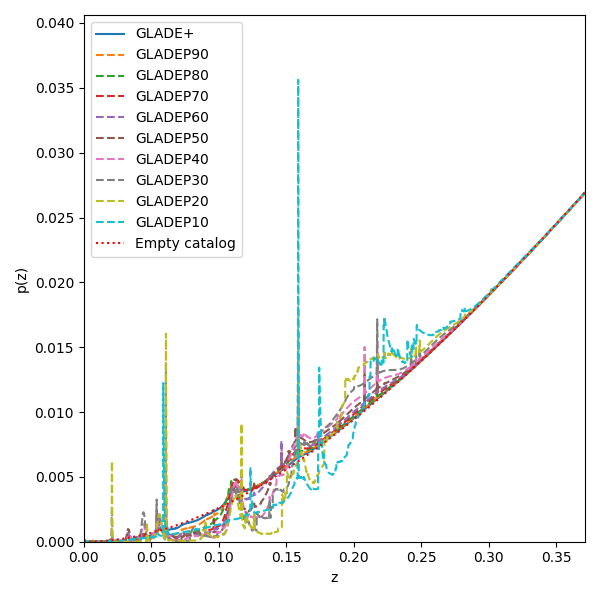
\includegraphics[width=0.7\textwidth]{figures/GW170809_zprior.png}
  \caption[LOS redshift prior for GW170809 for different brightness-ranked \texttt{GLADE} subsets]{LOS redshift prior for GW170809 for different brightness-ranked \texttt{GLADE} subsets. The full \texttt{GLADE+} catalog (solid blue) is compared to the different subsets. Applying a brightness cut amplifies the prior at higher distances, extending the effective reach of the catalog and partially mitigating incompleteness at greater redshifts.}
  \label{fig:los_prior_gw170809}
\end{figure}

\subsection{Hubble Constant Posterior}
Once one has the \ac{LOS} redshift prior, one can use it to compute the posterior distribution of the Hubble constant $H_0$ given the \ac{GW} event data, as the relation between the redhsift $z$, luminosity distance $d_L$ and the Hubble constant $H_0$ is given by:
\begin{align}
  d_L = \frac{c(1+z)}{H_0} \int_0^z \frac{dz'}{\sqrt{(1+z')^3\Omega_m + \Omega_\Lambda}}
\end{align}
for a flat $\Lambda$CDM cosmology. At lower redshifts, this can be simplified to:
\begin{align}
  d_L \approx \frac{cz}{H_0}
\end{align}
Thus the \ac{LOS} redshift prior, $p(z|\Omega_i, \Lambda, s, I)$, and the luminosity distance posterior, $p(d_L,\Omega\mid\mathrm{GW})$, from the \ac{GW} event data can be combined to obtain the posterior distribution of $H_0$, which can then be used to obtain constraints on the value of $H_0$.

\begin{figure}[h!]
  \centering
  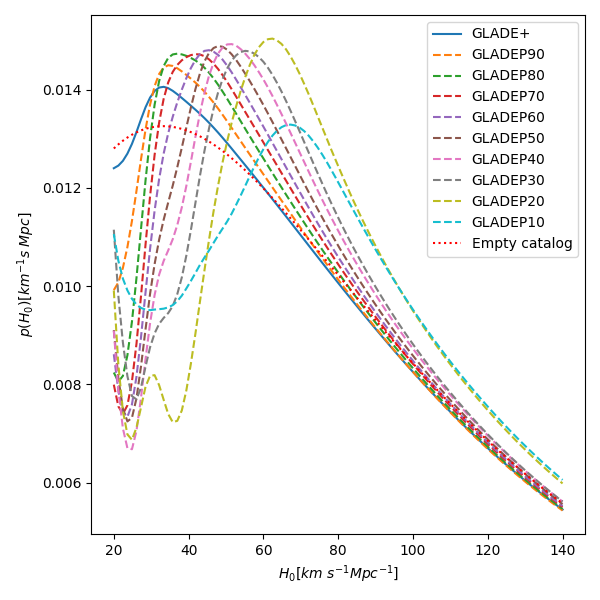
\includegraphics[width=0.7\textwidth]{figures/GW170809_H0.png}
  \caption[$H_0$ posterior distributions for GW170809 using full and brightness-cut galaxy catalogs.]{$H_0$ posterior distributions for GW170809 using full and brightness-cut galaxy catalogs. \texttt{GLADEP20} yields the tightest credible interval. \texttt{GLADEP10} suffers from sparse sampling.}
  \label{fig:h0_gw170809}
\end{figure}

Figure~\ref{fig:h0_gw170809} shows the resulting $H_0$ posteriors for GW170809 under various catalog cuts. As the catalog is restricted to brighter galaxies, the $H_0$ posterior becomes increasingly narrow. For example, \texttt{GLADEP20} yields a visibly tighter posterior compared to the full \texttt{GLADE+}, with minimal shift in the median. However, the most aggressive cut (\texttt{GLADEP10}) introduces broader tails, likely due to insufficient galaxy sampling in the localization volume. (\textbf{LINK TO THE 20\% LIMIT IN BUZZARD?})

We repeat this procedure for a subset of \ac{BBH} events from \ac{GWTC} that meet our selection criteria. Figure~\ref{fig:h0_cumulative} shows the combined $H_0$ posterior from the selected dark siren events using the full \texttt{GLADE+} catalog and the different subsets.

Table~\ref{tab:h0_stats} summarizes the $H_0$ posteriors for all cuts. The uncertainty is minimized around the \texttt{GLADEP20} subset, showing 30-40\% tighter contraints, while median values shift towards a higher value. For less extreme cuts, the median values doesn't show a huge shift. This suggests that moderate brightness cuts improve precision without introducing systematic bias.

\begin{figure}[ht]
    \centering
    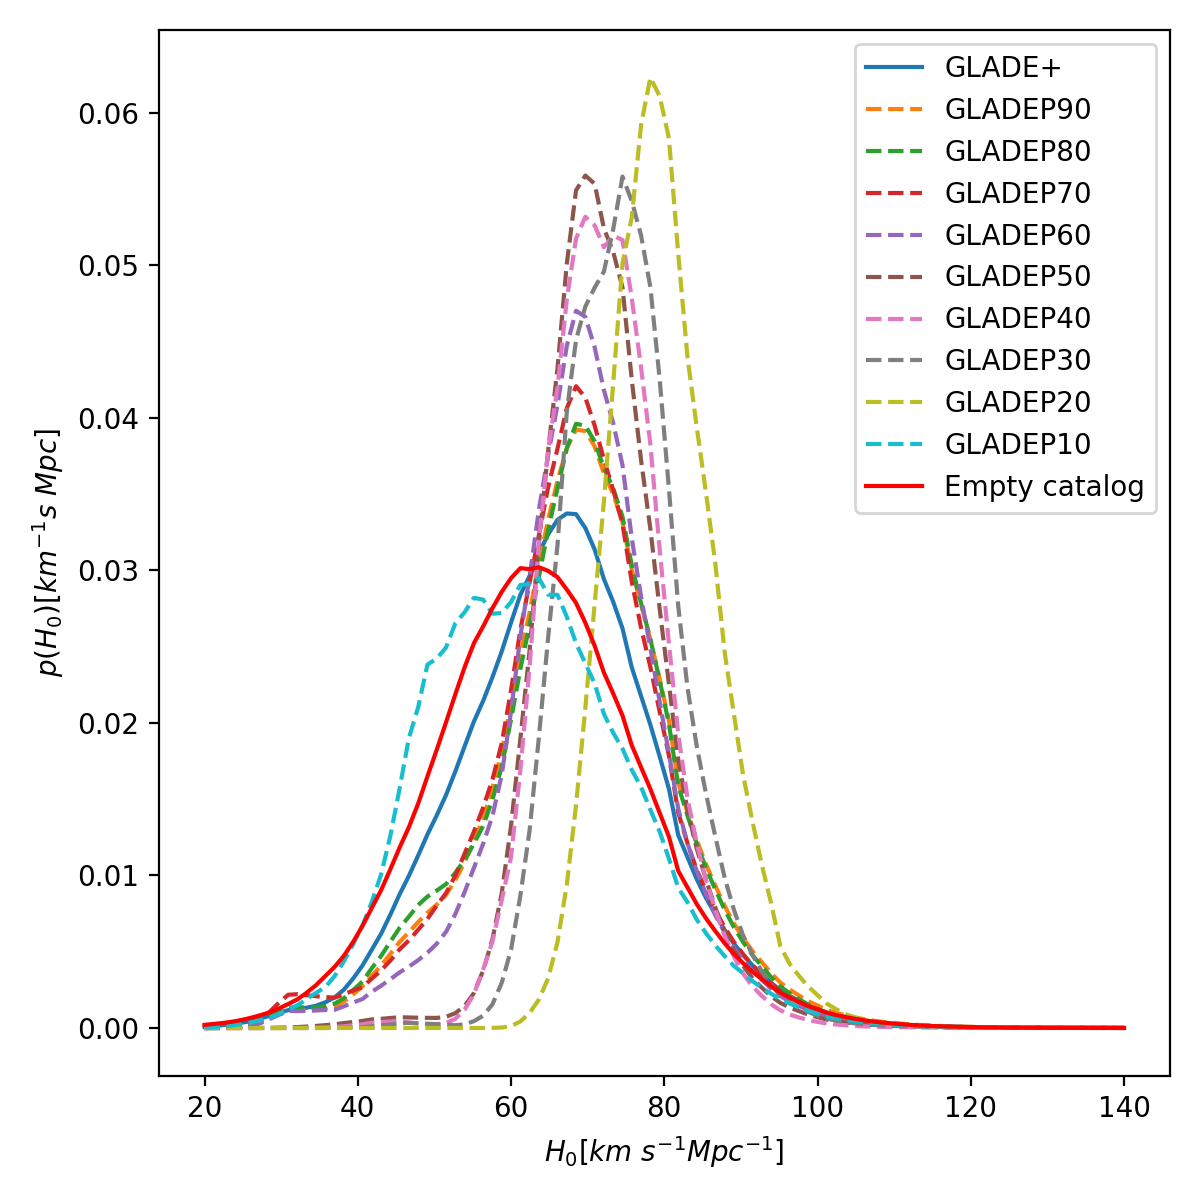
\includegraphics[width=0.7\textwidth]{figures/percentile_full_dict.png}
    \caption[Cumulative $H_0$ posterior from the slected dark siren events using full \texttt{GLADE+} and the different subsets.]{Cumulative $H_0$ posterior from the slected dark siren events using full \texttt{GLADE+} (blue) and the different subsets (dashed lines). The brightness-weighted catalog yields a tighter constraint without a significant shift.}
    \label{fig:h0_cumulative}
\end{figure}

\begin{table}
    \centering
    \caption[$H_0$ MAP values with $68\%$ confidence ranges, alongside the maximum magnitude limits for \texttt{GLADE+} and the different subsets.]{Maximum {\em a posteriori} probabilities with $68\%$ confidence ranges of the $H_0$ posterior distributions alongside the maximum magnitude limits for the different percentiles of the GLADE+ galaxy catalogue.}
    \begin{tabular}{c c c }
    \hline
        \textbf{Catalogue} & $M_{K, max}$ & $H_0~[km~s^{-1}Mpc^{-1}]$ \\ \hline
        \texttt{GLADE+} & -19.00 & $67.87^{+8.97}_{-10.29}$ \\
        \texttt{GLADEP90} & -23.07 & $68.94^{+9.24}_{-7.55}$ \\
        \texttt{GLADEP80} & -23.62 & $68.93^{+9.25}_{-7.57}$ \\
        \texttt{GLADEP70} & -23.94 & $68.63^{+8.61}_{-7.42}$ \\
        \texttt{GLADEP60} & -24.19 & $68.85^{+7.72}_{-6.43}$ \\
        \texttt{GLADEP50} & -24.14  & $70.05^{+6.12}_{-5.20}$ \\
        \texttt{GLADEP40} & -24.63 & $69.94^{+7.46}_{-3.88}$ \\
        \texttt{GLADEP30} & -24.87 & $74.70^{+4.69}_{-6.58}$ \\
        \texttt{GLADEP20} & -25.15 & $78.28^{+5.53}_{-4.95}$ \\
        \texttt{GLADEP10} & -25.53 & $63.46^{+6.39}_{-14.37}$ \\ \hline
    \end{tabular}
    \label{tab:h0_stats}
\end{table}

\subsection{Cost–benefit trade-off} 
We observe that precision improves with increasing brightness until an optimum is reached (near \texttt{GLADEP20}). Beyond this point, the posterior widens again, moving towards an empty catalog result, due to under-sampling. This defines a practical limit for catalog pruning. In real applications, the exact optimum may depend on event SNR, catalog completeness, and the merger rate model.

Our results suggest that targeting the brightest galaxies in a well-characterized catalog can substantially improve the statistical precision of $H_0$ constraints from dark sirens. This approach complements other efforts to mitigate catalog incompleteness, including joint inference with galaxy clustering and population-informed redshift estimation.
%\chapter{Results}
\label{chap:results}

In this chapter, we present the main results of our dark siren cosmology analysis using brightness-ranked subsets of the \texttt{GLADE+} galaxy catalog. We evaluate the impact of applying magnitude cuts on the galaxy sample, compare the resulting \ac{LOS} redshift priors, and show how these choices affect the posterior distribution of the Hubble constant $H_0$. We also assess the precision-bias trade-off associated with aggressive catalog cuts.

\section{LOS Redshit Prior}
The first step in our cosmological inference is computing the \ac{LOS} redshift prior $p(z | \Omega, \Lambda, s, I)$ for each \ac{GW} event and sky pixel $\Omega$. This prior combines the redshift distribution of galaxies in the \texttt{GLADE+} catalog with an analytic model for the out-of-catalog population, as described in Chapter~\ref{chap:methodology}.

To test the impact of catalog completeness, we apply successive cuts to the galaxy catalog by selecting only the brightest $XX\%$ of galaxies in $K$-band luminosity, forming subsets labeled \texttt{GLADEPXX}. This process shifts the effective magnitude threshold upward, reducing the number of galaxies but improving the catalog's completeness above the cut.

Figure~\ref{fig:los_prior_gw170809} shows the LOS redshift prior for the event GW170809 under different catalog cuts. Bright galaxy subsets (e.g., \texttt{GLADEP20}) result in sharper redshift distributions and reduce the weight of the out-of-catalog term. Notably, these priors maintain consistency in shape, indicating that bright galaxies are reliable tracers of large-scale structure. The application of a brightness cut significantly modifies the \ac{LOS} redshift distribution. Specifically, the bright galaxy subsets yield an amplified redshift prior at higher distances, effectively extending the reach of the catalogue, somewhat mitigating the incompleteness issues that arise at deeper redshifts.

\begin{figure}[ht]
    \centering
    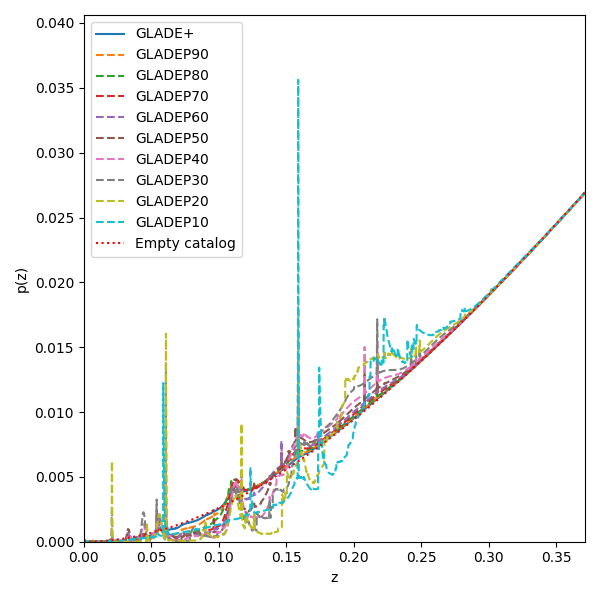
\includegraphics[width=0.7\textwidth]{figures/GW170809_zprior.png}
    \caption[LOS redshift prior for GW170809 for different brightness-ranked \texttt{GLADE} subsets]{LOS redshift prior for GW170809 for different brightness-ranked \texttt{GLADE} subsets. The full \texttt{GLADE+} catalog (solid blue) is compared to the different subsets. Applying a brightness cut amplifies the prior at higher distances, extending the effective reach of the catalog and partially mitigating incompleteness at greater redshifts.}
    \label{fig:los_prior_gw170809}
\end{figure}

\section{$H_0$ Posterior}

With \ac{LOS} priors in hand, we compute the posterior distribution for the Hubble constant $H_0$ by combining the GW posterior $p(d_L, \Omega | \text{GW})$ with the redshift prior $p(z | \Omega, \Lambda, s, I)$. This is done using the \texttt{gwcosmo} pipeline for each event.

Figure~\ref{fig:h0_gw170809} shows the resulting $H_0$ posteriors for GW170809 under various catalog cuts. As the catalog is restricted to brighter galaxies, the $H_0$ posterior becomes increasingly narrow. For example, GLADEP20 yields a visibly tighter posterior compared to the full GLADE+, with minimal shift in the median. However, the most aggressive cut (GLADEP10) introduces broader tails, likely due to insufficient galaxy sampling in the localization volume.

\begin{figure}[ht]
    \centering
    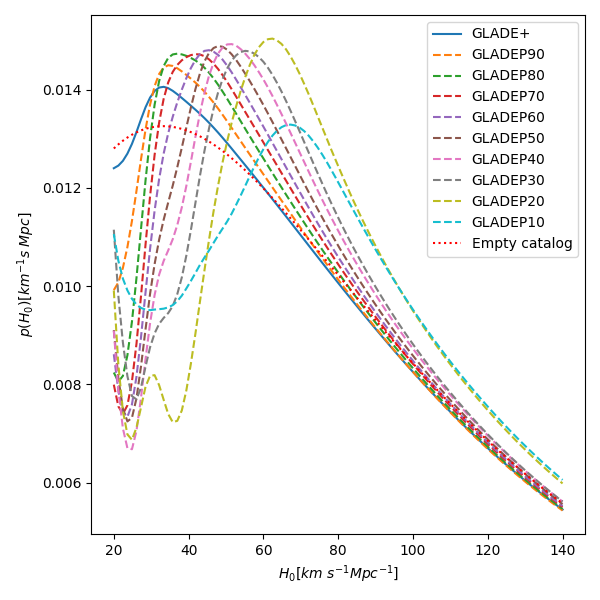
\includegraphics[width=0.7\textwidth]{figures/GW170809_H0.png}
    \caption[$H_0$ posterior distributions for GW170809 using full and brightness-cut galaxy catalogs.]{$H_0$ posterior distributions for GW170809 using full and brightness-cut galaxy catalogs. \texttt{GLADEP20} yields the tightest credible interval. \texttt{GLADEP10} suffers from sparse sampling.}
    \label{fig:h0_gw170809}
\end{figure}

We repeat this procedure for a subset of \ac{BBH} events from \ac{GWTC} that meet our selection criteria. Figure~\ref{fig:h0_cumulative} shows the combined $H_0$ posterior from the selected dark siren events using the full \texttt{GLADE+} catalog and the different subsets.

Table~\ref{tab:h0_stats} summarizes the $H_0$ posteriors for all cuts. The uncertainty is minimized around the \texttt{GLADEP20} subset, showing 30-40\% tighter contraints, while median values shift towards a higher value. For less extreme cuts, the median values doesn't show a huge shift. This suggests that moderate brightness cuts improve precision without introducing systematic bias.

\begin{figure}[ht]
    \centering
    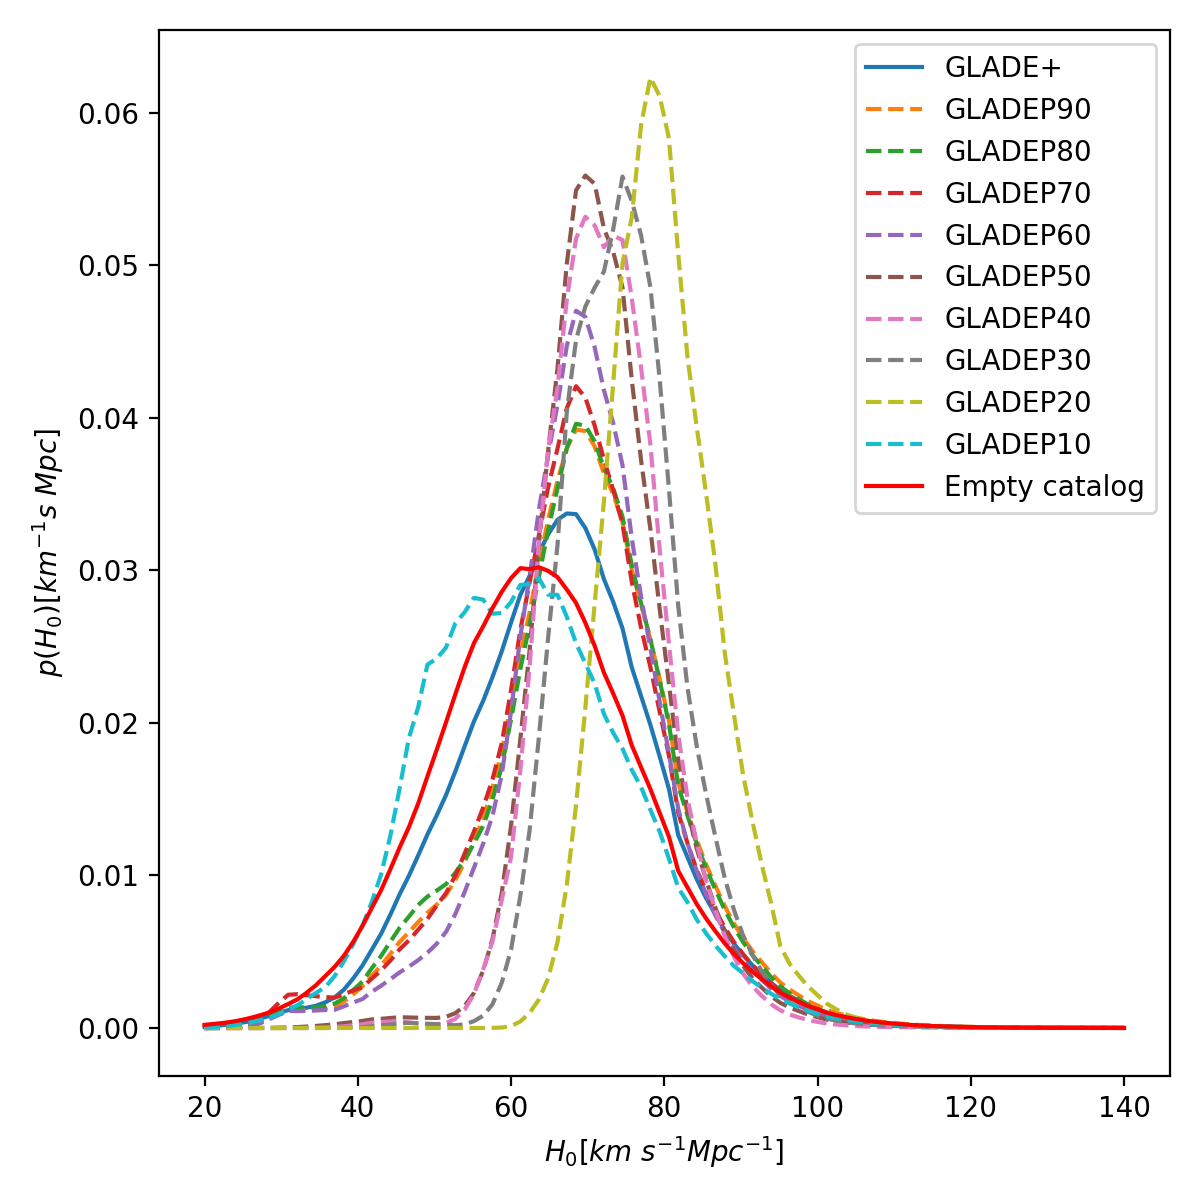
\includegraphics[width=0.7\textwidth]{figures/percentile_full_dict.png}
    \caption[Cumulative $H_0$ posterior from the slected dark siren events using full \texttt{GLADE+} and the different subsets.]{Cumulative $H_0$ posterior from the slected dark siren events using full \texttt{GLADE+} (blue) and the different subsets (dashed lines). The brightness-weighted catalog yields a tighter constraint without a significant shift.}
    \label{fig:h0_cumulative}
\end{figure}

\begin{table}
    \centering
    \caption[$H_0$ MAP values with $68\%$ confidence ranges, alongside the maximum magnitude limits for \texttt{GLADE+} and the different subsets.]{Maximum {\em a posteriori} probabilities with $68\%$ confidence ranges of the $H_0$ posterior distributions alongside the maximum magnitude limits for the different percentiles of the GLADE+ galaxy catalogue.}
    \begin{tabular}{c c c }
    \hline
        \textbf{Catalogue} & \textbf{$M_{K, max}$} & \textbf{$H_0~[km~s^{-1}Mpc^{-1}]$} \\ \hline
        \texttt{GLADE+} & -19.00 & $67.87^{+8.97}_{-10.29}$ \\
        \texttt{GLADEP90} & -23.07 & $68.94^{+9.24}_{-7.55}$ \\
        \texttt{GLADEP80} & -23.62 & $68.93^{+9.25}_{-7.57}$ \\
        \texttt{GLADEP70} & -23.94 & $68.63^{+8.61}_{-7.42}$ \\
        \texttt{GLADEP60} & -24.19 & $68.85^{+7.72}_{-6.43}$ \\
        \texttt{GLADEP50} & -24.14  & $70.05^{+6.12}_{-5.20}$ \\
        \texttt{GLADEP40} & -24.63 & $69.94^{+7.46}_{-3.88}$ \\
        \texttt{GLADEP30} & -24.87 & $74.70^{+4.69}_{-6.58}$ \\
        \texttt{GLADEP20} & -25.15 & $78.28^{+5.53}_{-4.95}$ \\
        \texttt{GLADEP10} & -25.53 & $63.46^{+6.39}_{-14.37}$ \\ \hline
    \end{tabular}
    \label{tab:h0_stats}
\end{table}

\section{Cost–benefit trade-off}
We observe that precision improves with increasing brightness until an optimum is reached (near \texttt{GLADEP20}). Beyond this point, the posterior widens again due to under-sampling. This defines a practical limit for catalog pruning. In real applications, the exact optimum may depend on event SNR, catalog completeness, and the merger rate model.

Our results suggest that targeting the brightest galaxies in a well-characterized catalog can substantially improve the statistical precision of $H_0$ constraints from dark sirens. This approach complements other efforts to mitigate catalog incompleteness, including joint inference with galaxy clustering and population-informed redshift estimation.
\chapter{Mock Data Challenge}
\label{chap:MDC}

\section{BUZZARD Mock Catalog}

\section{GWSim}

\section{Results}
%\chapter{Discussion}
\label{chap:discussion}
\chapter{Conclusion}
\label{chap:conclusion}

The emergence of \ac{GW} astronomy has opened a new frontier in observational cosmology. This thesis has explored the potential of using dark sirens, gravitational-wave events without electromagnetic counterparts, for the inference of the Hubble constant, $H_0$. Specifically, we examined whether refining the galaxy catalog used in the redshift prior, by restricting it to its brightest subsets, can improve the cosmological constraints from these events.

\section{Summary of Findings}

We implemented a hierarchical Bayesian inference framework using the \texttt{gwcosmo} pipeline, which combines \ac{GW} luminosity distance posteriors with redshift priors constructed from galaxy catalogs. The galaxy redshift prior was derived using the \texttt{GLADE+} catalog and modified by applying brightness cuts to prioritize the most luminous galaxies in the $K$-band. These subsets, denoted \texttt{GLADEPXX}, were hypothesized to trace large-scale structure more efficiently due to their association with massive halos.

The analysis demonstrated that:
\vspace{-1em}
\begin{itemize}
    \item Brightness-ranked catalogs improve the redshift prior, leading to tighter posteriors on $H_0$ by reducing low-likelihood host candidates in the \ac{GW} localization volume.
    \vspace{-1em}
    \item Moderate pruning yields improvement in $H_0$ precision as compared to using the full catalog, without introducing measurable bias. This improvement is attributed to the enhanced clustering signal from retaining mostly central, high-luminosity galaxies.
    \vspace{-1em}
    \item Aggressive pruning (e.g., \texttt{GLADEP10}) results in degraded constraints and larger uncertainties, as the catalog no longer adequately traces the large-scale structure.
    \vspace{-1em}
    \item A lower bound of approximately 30\% of the brightest galaxies emerges as a practical pruning limit, in the best-case scenario where the brightest galaxies are strictly the central-most galaxies. Below this threshold, significant information about the underlying matter distribution is lost, particularly from central galaxies, increasing the risk of cosmological bias.
    \vspace{-1em}
    \item Simulated mock challenges using the \texttt{BUZZARD} catalog support the robustness of the brightness-based pruning strategy but also emphasize the importance of catalog completeness, redshift depth, and optimal percentile thresholds. The 30\% structural limit appears consistent across magnitude cuts, suggesting that future work should avoid overly aggressive pruning or instead develop hybrid approaches combining full and pruned catalogs.
\end{itemize}

\section{Limitations}

This work, while comprehensive, has several limitations:
\vspace{-1em}
\begin{itemize}
    \item The number of \ac{GW} events with high \ac{SNR} and good localization remains small, limiting the statistical power of our results.
    \vspace{-1em}
    \item Catalog incompleteness, particularly at high redshifts, introduces uncertainties that are only partially mitigated by brightness cuts.
    \vspace{-1em}
    \item Due to time constraints and several technical challenges encountered with the \texttt{BUZZARD} mock catalog, we were unable to perform a full end-to-end bias quantification from pruning dim galaxies. Nevertheless, partial analyses and theoretical considerations support the proposed 30\% threshold as a conservative lower bound.
    \vspace{-1em}
    \item While a complete end-to-end \acf{MDC} framework has been developed, a few components still require minor refinements and consistency checks before full deployment in future analyses.
    %\vspace{-1em}
    %\item The analysis assumes a fixed $\Lambda$CDM cosmology throughout, exploring extended models may reveal different degeneracies or sensitivities in dark siren inference.
\end{itemize}

\section{Outlook and Future Work}

The outlook for dark siren cosmology is highly promising. With the advent of next-generation \ac{GW} detectors such as Cosmic Explorer~\citep{Evans:CE}, Einstein Telescope~\citep{Abac:ET} and LISA~\citep{LISA:2024hlh}, and deeper galaxy surveys (e.g., LSST~\citep{ivezic2019lsst}, Euclid~\citep{mellier2024euclid}), both the number of detected events and the completeness of host catalogs are expected to improve significantly.

Future extensions of this work could include:
\vspace{-1em}
\begin{itemize}
    \item Get a quantitative estimate of the bias introduced by the brightness cuts, with the devised end-to-end \ac{MDC} framework.
    \vspace{-1em}
    \item Testing for potential biases introduced by brightness cuts using larger and more realistic mock datasets.
    \vspace{-1em}
    \item Developing adaptive redshift priors that vary with localization volume depth, combining full catalogs at low redshift with bright subsets at high redshift.
    \vspace{-1em}
    \item Integrating clustering information or cross-correlations with large-scale structure to improve redshift inference~\citep{afroz2024prospect}.
\end{itemize}

Ultimately, the resolution of the Hubble tension will require a convergence of multiple independent probes. As shown in this thesis, dark sirens, when carefully analyzed, offer a robust and independent route to measuring $H_0$. Furthermore, the use of bright galaxies as tracers of large-scale structure provides a promising avenue for improving the precision of cosmological constraints from \ac{GW} observations. This methodology will play a growing role in the era of multi-messenger cosmology.

\cleardoublepage

% --------------------------
% Back matter
% --------------------------

\setstretch{1.1}
\renewcommand{\bibfont}{\normalfont\small}
\setlength{\biblabelsep}{0pt}
\setlength{\bibitemsep}{0.5\baselineskip plus 0.5\baselineskip}
\printbibliography
\cleardoublepage

% **************************************************
% End of Document CONTENT
% **************************************************
\end{document}
